\chapter{Risultati}
\label{sec:results}

% Source notes: Project/docs/thesis_notes.md (Ch. 6) and checkpoint_2026-10-10.md. Numbers:
% Project/outputs/results/<run>/{t1,t2,t3,calibration,latency,energy}/metrics.json; bootstrap: results/bootstrap/summary.md.
% Figures: Project/outputs/figures/{benchmarks,bootstrap,training-*,calibration-*}/ (copied to Thesis/images/results/).

Questo capitolo riporta i risultati sperimentali. Si parte da come GroundOne apprende il task e da quanto il suo
addestramento sia stabile. Seguono i risultati sui tre test set congelati, il confronto con le baseline e il contributo
che il readout del decision model dà di per sé. Il capitolo esamina poi la qualità delle probabilità, anche a confronto con giudici LLM che producono lo stesso output, il tempo e l'energia necessari per verificare una risposta, le misure di località (esecuzione offline, quantizzazione e co-residenza) e, infine, gli errori che restano. Gli intervalli, riportati tra parentesi nella
forma ``da $a$ a $b$'', sono intervalli di confidenza al 95\,\% ottenuti con un bootstrap a cluster, calcolati come
descritto nella Sezione~\ref{sec:setup-statistics}. La Figura~\ref{fig:results-bootstrap} raccoglie in un unico grafico le differenze appaiate discusse nel capitolo.

\begin{figure}[htbp]
\centering
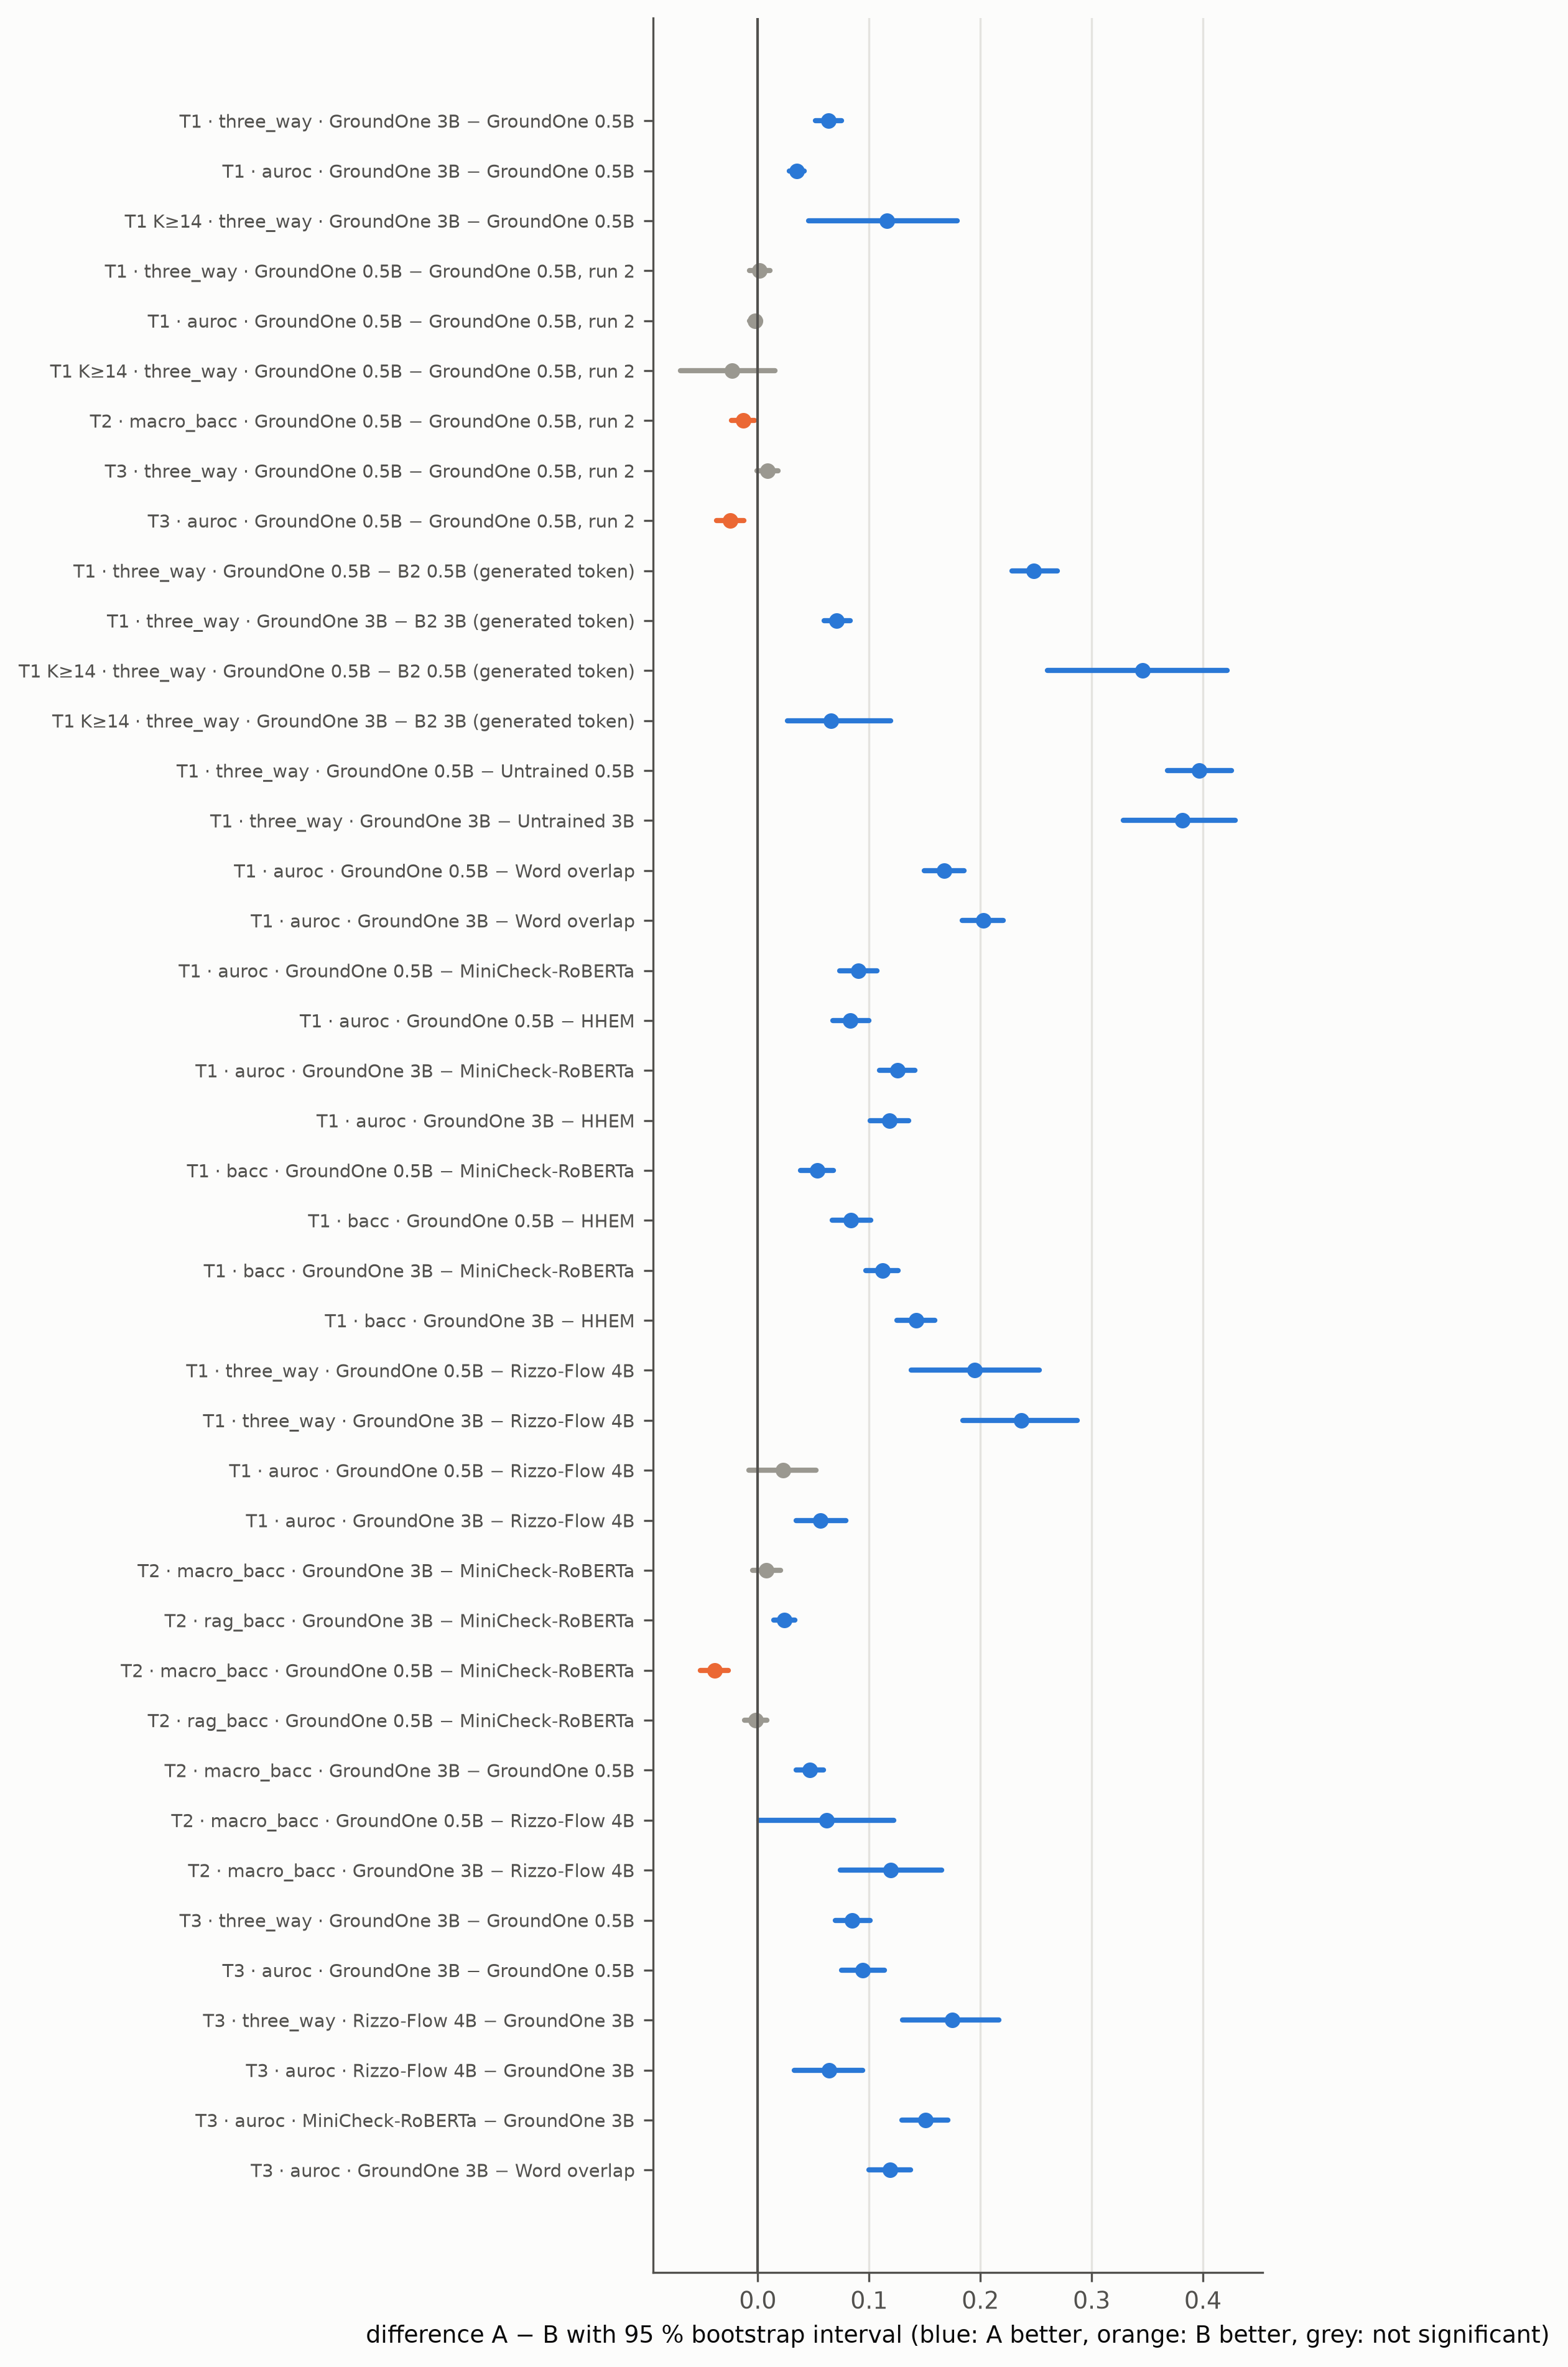
\includegraphics[width=\textwidth]{images/results/bootstrap_paired_differences.png}
\caption{Tutte le differenze appaiate tra sistemi sui test set congelati, con l'intervallo bootstrap a cluster al 95\,\%. In blu le differenze a favore del primo sistema (A), in arancione quelle a favore del secondo (B), in grigio quelle non significative, il cui intervallo contiene lo zero.}
\label{fig:results-bootstrap}
\end{figure}

\section{Addestramento}
\label{sec:results-training}

Entrambi i modelli hanno appreso il task. Prima dell'addestramento, un modello che riceve il formato con i marker non sa
che cosa il marker gli chieda, e i suoi verdetti sono casuali: il 0.5B risponde ``contraddetta'' per l'88\,\% delle frasi
del dev set e raggiunge una balanced accuracy a tre classi di 0.32. Nelle esecuzioni completate, invece, la loss di
addestramento è scesa già nei primi cento passi sotto il valore di un modello che conosca soltanto le frequenze delle
classi ($\ln 3 \approx 1.10$), e il punteggio sul dev set è poi cresciuto con regolarità (Figura~\ref{fig:results-dev}).

Il 0.5B è stato addestrato su tutte le 13{,}203 risposte e ha raggiunto il punteggio migliore al passo 600 di 802, con
una balanced accuracy media sui tre task di 0.633; da quel punto in poi il punteggio si è stabilizzato. Il 3B, addestrato
per 12.25 ore su 6{,}500 risposte, ha raggiunto 0.705 al passo 320 di 403, misurato sul proprio sottoinsieme del dev set.
Sull'intero dev set la balanced accuracy a tre classi è di 0.731 per il 0.5B e di 0.784 per il 3B. In entrambe le
esecuzioni, inoltre, tutte e tre le classi sono rimaste presenti fra le predizioni per tutta la durata
dell'addestramento.

\begin{figure}[htbp]
\centering
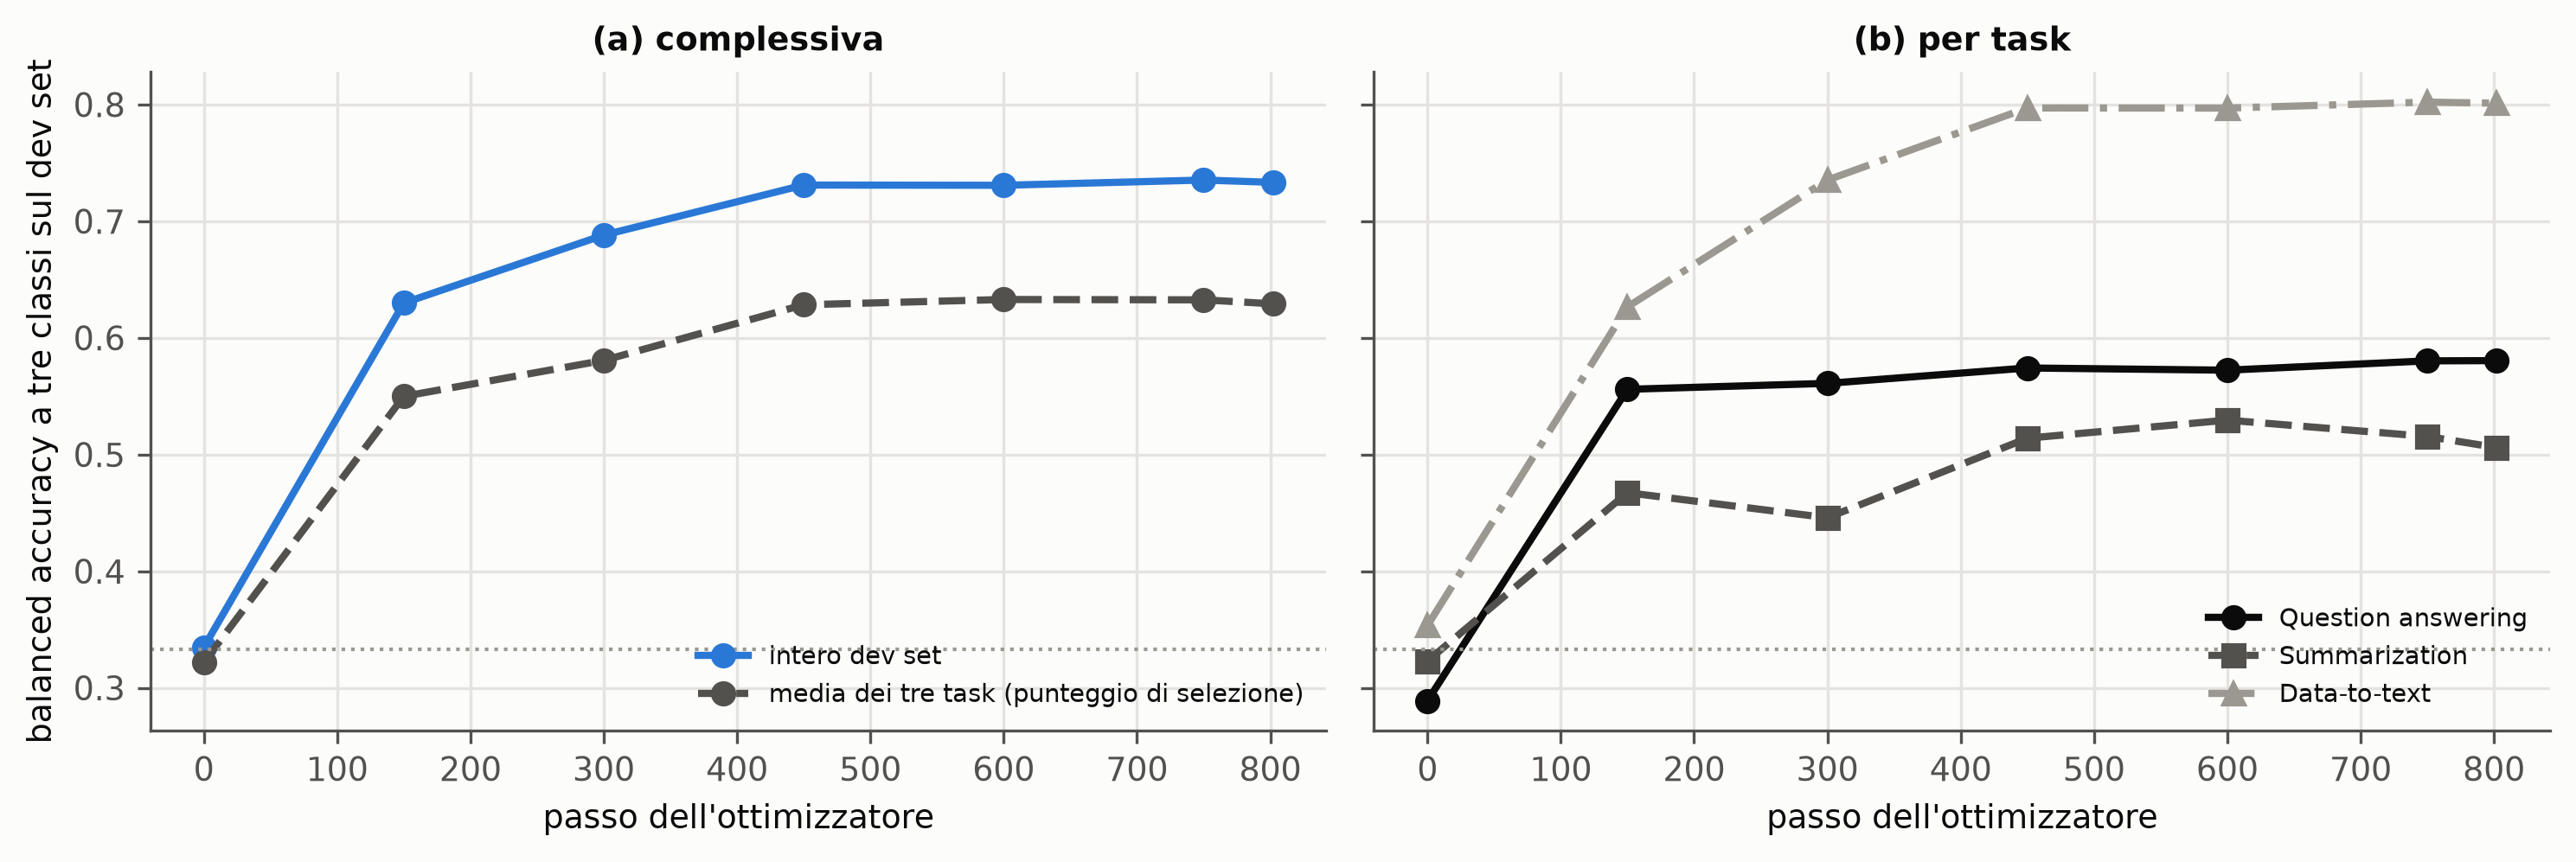
\includegraphics[width=\textwidth]{images/results/g1-05b-dev_bacc.png}
\caption{Balanced accuracy a tre classi sul dev set durante l'addestramento del modello 0.5B: valore complessivo (a
sinistra) e valore per task (a destra). La linea punteggiata indica il livello casuale. Il 3B mostra lo stesso andamento
sul proprio sottoinsieme di 200 risposte del dev set.}
\label{fig:results-dev}
\end{figure}

\section{Variabilità tra seed}
\label{sec:results-seeds}

Per capire quanto i risultati dipendano dal seed, la procedura del 0.5B è stata ripetuta con un secondo seed, che cambia
l'inizializzazione degli adapter e l'ordine dei batch. Quando l'addestramento converge, converge allo stesso punto
(Figura~\ref{fig:results-seeds}). Su T1 la seconda esecuzione raggiunge una balanced accuracy a tre classi di 0.767,
contro 0.769 della prima, e un AUROC di 0.907 contro 0.905. Su LLM-AggreFact la balanced accuracy media macro è 71.5
contro 70.1, e su VitaminC la balanced accuracy a tre classi è 0.434 contro 0.442. Su T1 la differenza appaiata tra le
due esecuzioni, calcolata come prima meno seconda, è $+0.001$ (da $-0.008$ a $+0.012$) e non è significativa.

Le differenze emergono nei dettagli. Anzitutto, gli errori si distribuiscono in modo diverso tra le classi: la recall
delle frasi supportate e quella delle frasi non menzionate si spostano di circa 0.04, in direzioni opposte. Inoltre, le
porzioni più piccole dei dati oscillano di più. La balanced accuracy della fascia con quattordici o più decisioni varia
di 0.023, l'AUROC su VitaminC di 0.025, e i singoli dataset di LLM-AggreFact variano fino a dieci punti, come WiCE (67.9
contro 78.0).

\begin{figure}[htbp]
\centering
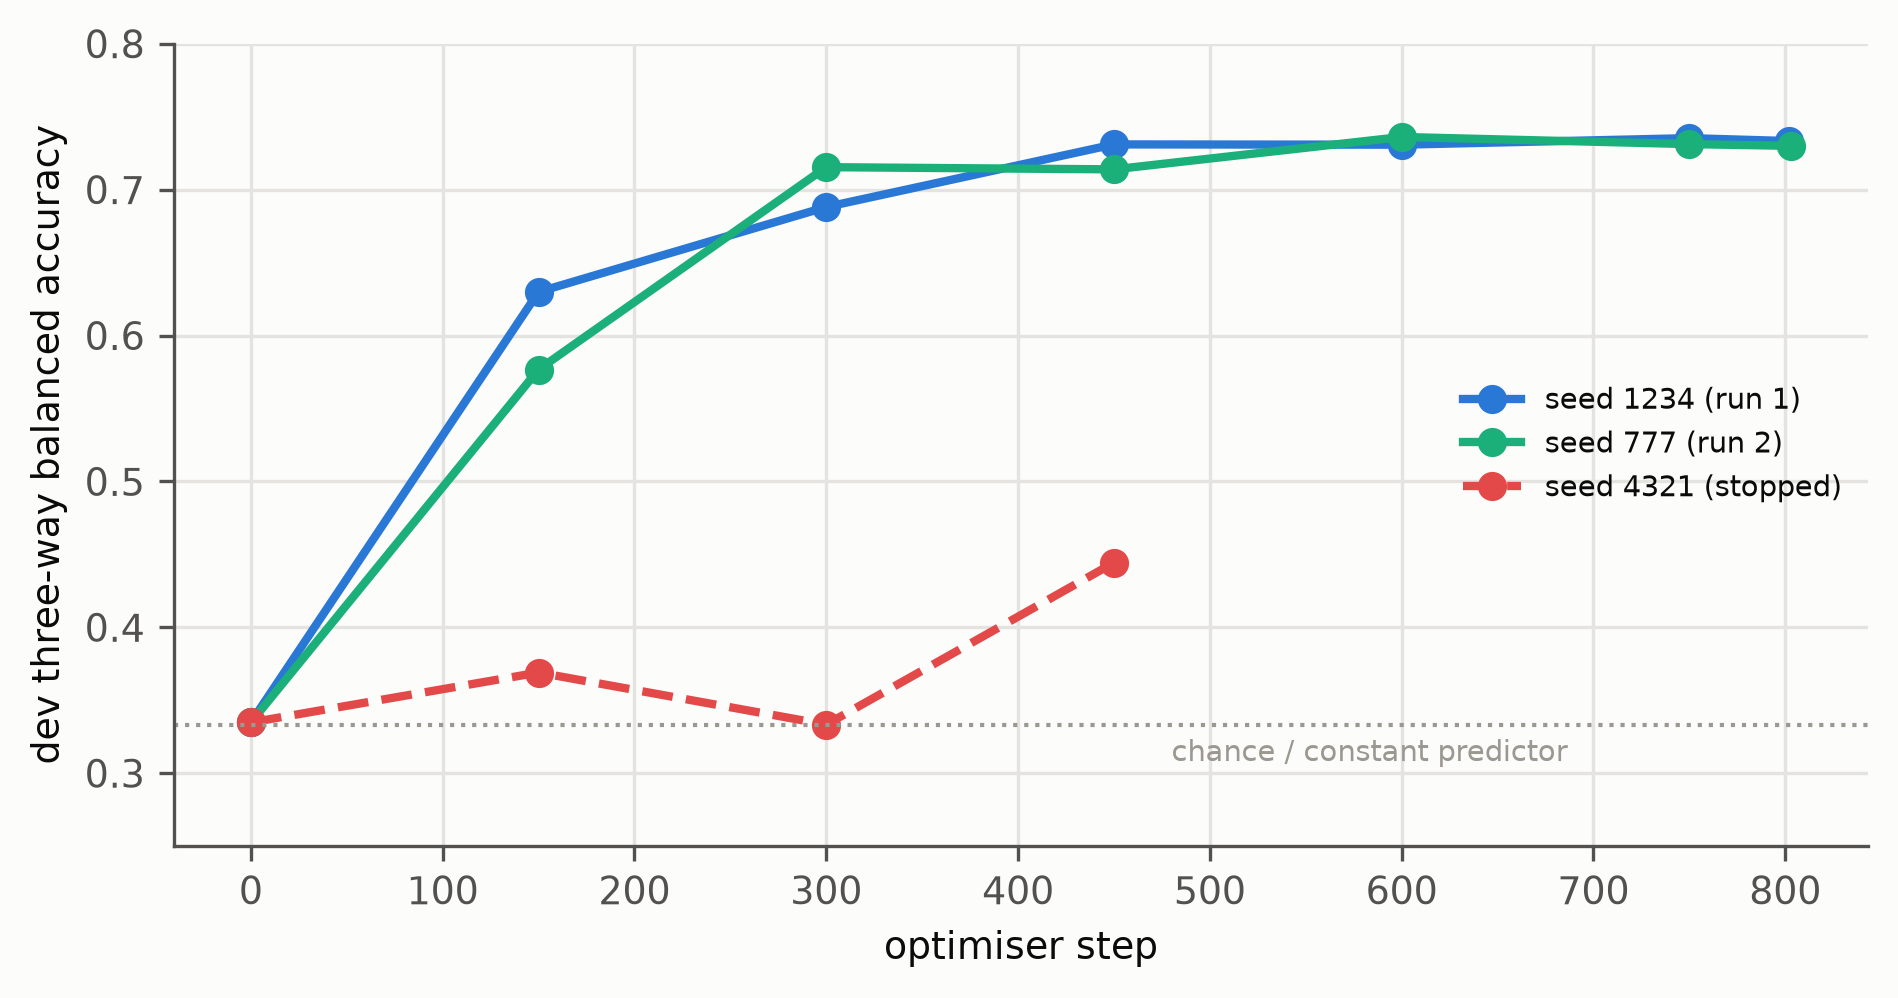
\includegraphics[width=0.85\textwidth]{images/results/seed_runs_05b.png}
\caption{Balanced accuracy a tre classi sul dev set durante l'addestramento del modello 0.5B, con la stessa procedura e
tre seed diversi. Due esecuzioni convergono allo stesso livello; la terza è collassata su un predittore costante ed è
stata interrotta.}
\label{fig:results-seeds}
\end{figure}

Da questi risultati seguono due conseguenze. La prima riguarda gli intervalli: il bootstrap ricampiona i dati di test,
e quindi non coglie la variabilità dovuta all'addestramento. Su LLM-AggreFact e su VitaminC, infatti, le due esecuzioni
della stessa procedura differiscono più di quanto i loro intervalli consentirebbero (prima meno seconda esecuzione: $-1.3$ punti sulla media macro di T2,
$-0.025$ sull'AUROC di T3). Per questo non vengono interpretate le differenze tra sistemi inferiori alla dispersione tra
seed, cioè a circa 1.5 punti sulla media macro di LLM-AggreFact e a 0.025 di AUROC su VitaminC. Lo stesso vale per i
singoli dataset di LLM-AggreFact quando lo scarto non supera circa cinque punti.

La seconda conseguenza è che l'addestramento non sempre converge. Un'esecuzione con un terzo seed è rimasta vicina al
livello casuale. Il suo punteggio sul dev set era 0.369 al passo 150 e 0.333 al passo 300, quando il modello prediceva
``supportata'' per ogni frase, e la loss di addestramento è rimasta prossima a quella di un modello privo di
informazione. Al passo 450 il punteggio era risalito a 0.444, e l'esecuzione è stata interrotta poco dopo, al passo 470 circa di 801. Non è quindi
possibile sapere se si sarebbe ripresa entro la fine dell'epoca e, poiché incompleta, è esclusa dalle tabelle. La
procedura ha due caratteristiche note per rendere fragile il fine-tuning: non applica gradient clipping, e
l'ottimizzatore lavora senza bias correction. L'assenza della bias correction è l'impostazione predefinita del framework
ed è stata indicata come una delle cause principali dei fine-tuning non
riusciti~\cite{pascanu2013difficulty,mosbach2021stability}. Un solo collasso su tre esecuzioni non basta a stimare un
tasso di fallimento, ma mostra che la procedura non è del tutto robusta rispetto all'inizializzazione.

\section{Accuratezza sul test set RAG (T1)}
\label{sec:results-t1}

Sulle 17{,}284 frasi di T1 il modello 0.5B raggiunge una balanced accuracy a tre classi di 0.769 e il 3B di 0.832
(Tabella~\ref{tab:results-t1}). La differenza tra i due, $+0.063$ (da $+0.051$ a $+0.076$), è l'effetto più netto della
dimensione del modello. Sulla decisione binaria il 0.5B ottiene una balanced accuracy di 0.815 e un AUROC di 0.905,
mentre il 3B ottiene rispettivamente 0.874 e 0.940. Entrambi superano di gran lunga i segnali che non confrontano mai una
frase con il suo documento: la sovrapposizione lessicale arriva a un AUROC di 0.737, e il classificatore che vede
soltanto la frase arriva a una balanced accuracy a tre classi di 0.570.

\begin{table}[htbp]
\centering
\caption{GroundOne su T1, sull'intero test set, per task e per numero di decisioni per risposta ($K$). Per ciascun
modello sono riportate la balanced accuracy a tre classi, la recall delle frasi contraddette e l'AUROC di $P(\text{supported})$. $^{*}$Valore indicativo: la cella contiene meno di 30 frasi contraddette.}
\label{tab:results-t1}
\small
\begin{adjustbox}{max width=\textwidth}
\begin{tabular}{@{}lrrrrrrr@{}}
\toprule
 & & \multicolumn{3}{c}{GroundOne 0.5B} & \multicolumn{3}{c}{GroundOne 3B} \\
\cmidrule(lr){3-5}\cmidrule(l){6-8}
Sottoinsieme & Frasi & Bal.\ acc. & Contr. & AUROC & Bal.\ acc. & Contr. & AUROC \\
\midrule
Tutte & 17{,}284 & 0.769 & 0.68 & 0.905 & 0.832 & 0.76 & 0.940 \\
\midrule
Question answering & 4{,}876 & 0.589 & 0.03$^{*}$ & 0.916 & 0.699 & 0.30$^{*}$ & 0.948 \\
Summarization & 4{,}538 & 0.544 & 0.13 & 0.775 & 0.629 & 0.30 & 0.873 \\
Data-to-text & 7{,}870 & 0.812 & 0.84 & 0.929 & 0.873 & 0.90 & 0.955 \\
\midrule
$K$ = 1--4 & 2{,}434 & 0.606 & 0.18 & 0.857 & 0.677 & 0.25 & 0.921 \\
$K$ = 5--8 & 8{,}012 & 0.758 & 0.67 & 0.899 & 0.829 & 0.78 & 0.936 \\
$K$ = 9--13 & 5{,}201 & 0.824 & 0.82 & 0.926 & 0.863 & 0.86 & 0.945 \\
$K \geq 14$ & 1{,}637 & 0.723 & 0.50 & 0.908 & 0.839 & 0.68 & 0.957 \\
\bottomrule
\end{tabular}
\end{adjustbox}
\end{table}

Dalla tabella emergono tre aspetti. Il primo è che l'accuratezza non crolla con la lunghezza della risposta. Le risposte con quattordici o più decisioni raggiungono una balanced accuracy di 0.839 con il 3B, tra le migliori, e di 0.723 con il 0.5B, leggermente al di sotto delle fasce intermedie. La fascia più difficile è invece quella delle risposte più brevi, che comprende soprattutto risposte
di question answering e di summarization. Il dato è importante perché è proprio sulle risposte lunghe che un decision model
fa risparmiare più tempo; su queste risposte il 3B guadagna sul 0.5B $+0.116$ (da $+0.053$ a $+0.186$).

Il secondo aspetto è che le contraddizioni vengono riconosciute soprattutto nel data-to-text, il task in cui RAGTruth le
concentra. Nel question answering e nella summarization il 0.5B distingue bene le frasi supportate da quelle non
menzionate, ma non individua quasi nessuna contraddizione: la recall delle frasi contraddette è 0.03 e 0.13, e il primo valore è solo indicativo, perché nel question answering le frasi contraddette sono meno di 30. Il 3B la
porta a 0.30 in entrambi i task, quindi la dimensione del modello compensa in parte la scarsità di questi esempi nei
dati di addestramento. Il terzo aspetto è che question answering e summarization offrono la prova più chiara che i
modelli leggono davvero il documento. In questi due task il classificatore che vede soltanto la frase resta al livello
casuale (0.36 e 0.35), mentre i due modelli raggiungono 0.59--0.70 nel question answering e 0.54--0.63 nella
summarization.

Le stesse predizioni si possono valutare anche a livello di risposta intera. È il criterio con cui il Decision Index
della comunità valuta i decision model generalisti su RAGTruth: una risposta è allucinata se contiene un qualsiasi
contenuto non supportato, e la metrica è l'F1 di questa classe. Un sistema che risponda sempre ``allucinata'' raggiunge
già un F1 di 0.52~\cite{decisionindex2026}. Per giudicare una risposta, GroundOne prende il minimo della
$P(\text{supported})$ calibrata sulle sue frasi e lo confronta con una soglia stimata sul dev set. Con questa regola,
sulle 2{,}647 risposte di T1 raggiunge un F1 di 0.733 con il 0.5B e di 0.784 con il 3B. Nella leaderboard, invece,
nessun decision model generalista sotto il miliardo di parametri supera 0.553, Jev raggiunge 0.765 e il modello migliore,
da 27B parametri, 0.803. Il confronto è solo indicativo, perché GroundOne è stato addestrato su RAGTruth, mentre i
modelli della leaderboard sono valutati zero-shot, con un prompt diverso e su 53 risposte in più. Colloca comunque uno
specialista da 0.5B molto al di sopra dei decision model generalisti della stessa dimensione.

\section{Confronto con le baseline}
\label{sec:results-baselines}

La Figura~\ref{fig:results-comparison} mette a confronto tutti i sistemi su T1. Gli encoder specializzati raggiungono un
AUROC di 0.814 (MiniCheck-RoBERTa) e di 0.821 (HHEM): più della sovrapposizione lessicale, ma meno di entrambi i modelli
GroundOne. Il 0.5B supera MiniCheck-RoBERTa di $+0.091$ (da $+0.074$ a $+0.108$) e HHEM di $+0.083$ (da $+0.067$ a
$+0.099$); il 3B li supera rispettivamente di $+0.126$ e $+0.119$. Il confronto per task, però, ridimensiona questo
risultato. Il vantaggio di GroundOne viene in gran parte dal data-to-text, dove lo avvantaggiano l'addestramento nel dominio e la struttura ricorrente dei template, e dove gli
encoder sono più deboli (AUROC 0.71--0.75). Nella summarization, invece, MiniCheck-RoBERTa supera il modello 0.5B (0.872
contro 0.775) ed è alla pari con il 3B (0.873). La Figura~\ref{fig:results-by-task} riporta l'AUROC per task di tutti i sistemi.

\begin{figure}[htbp]
\centering
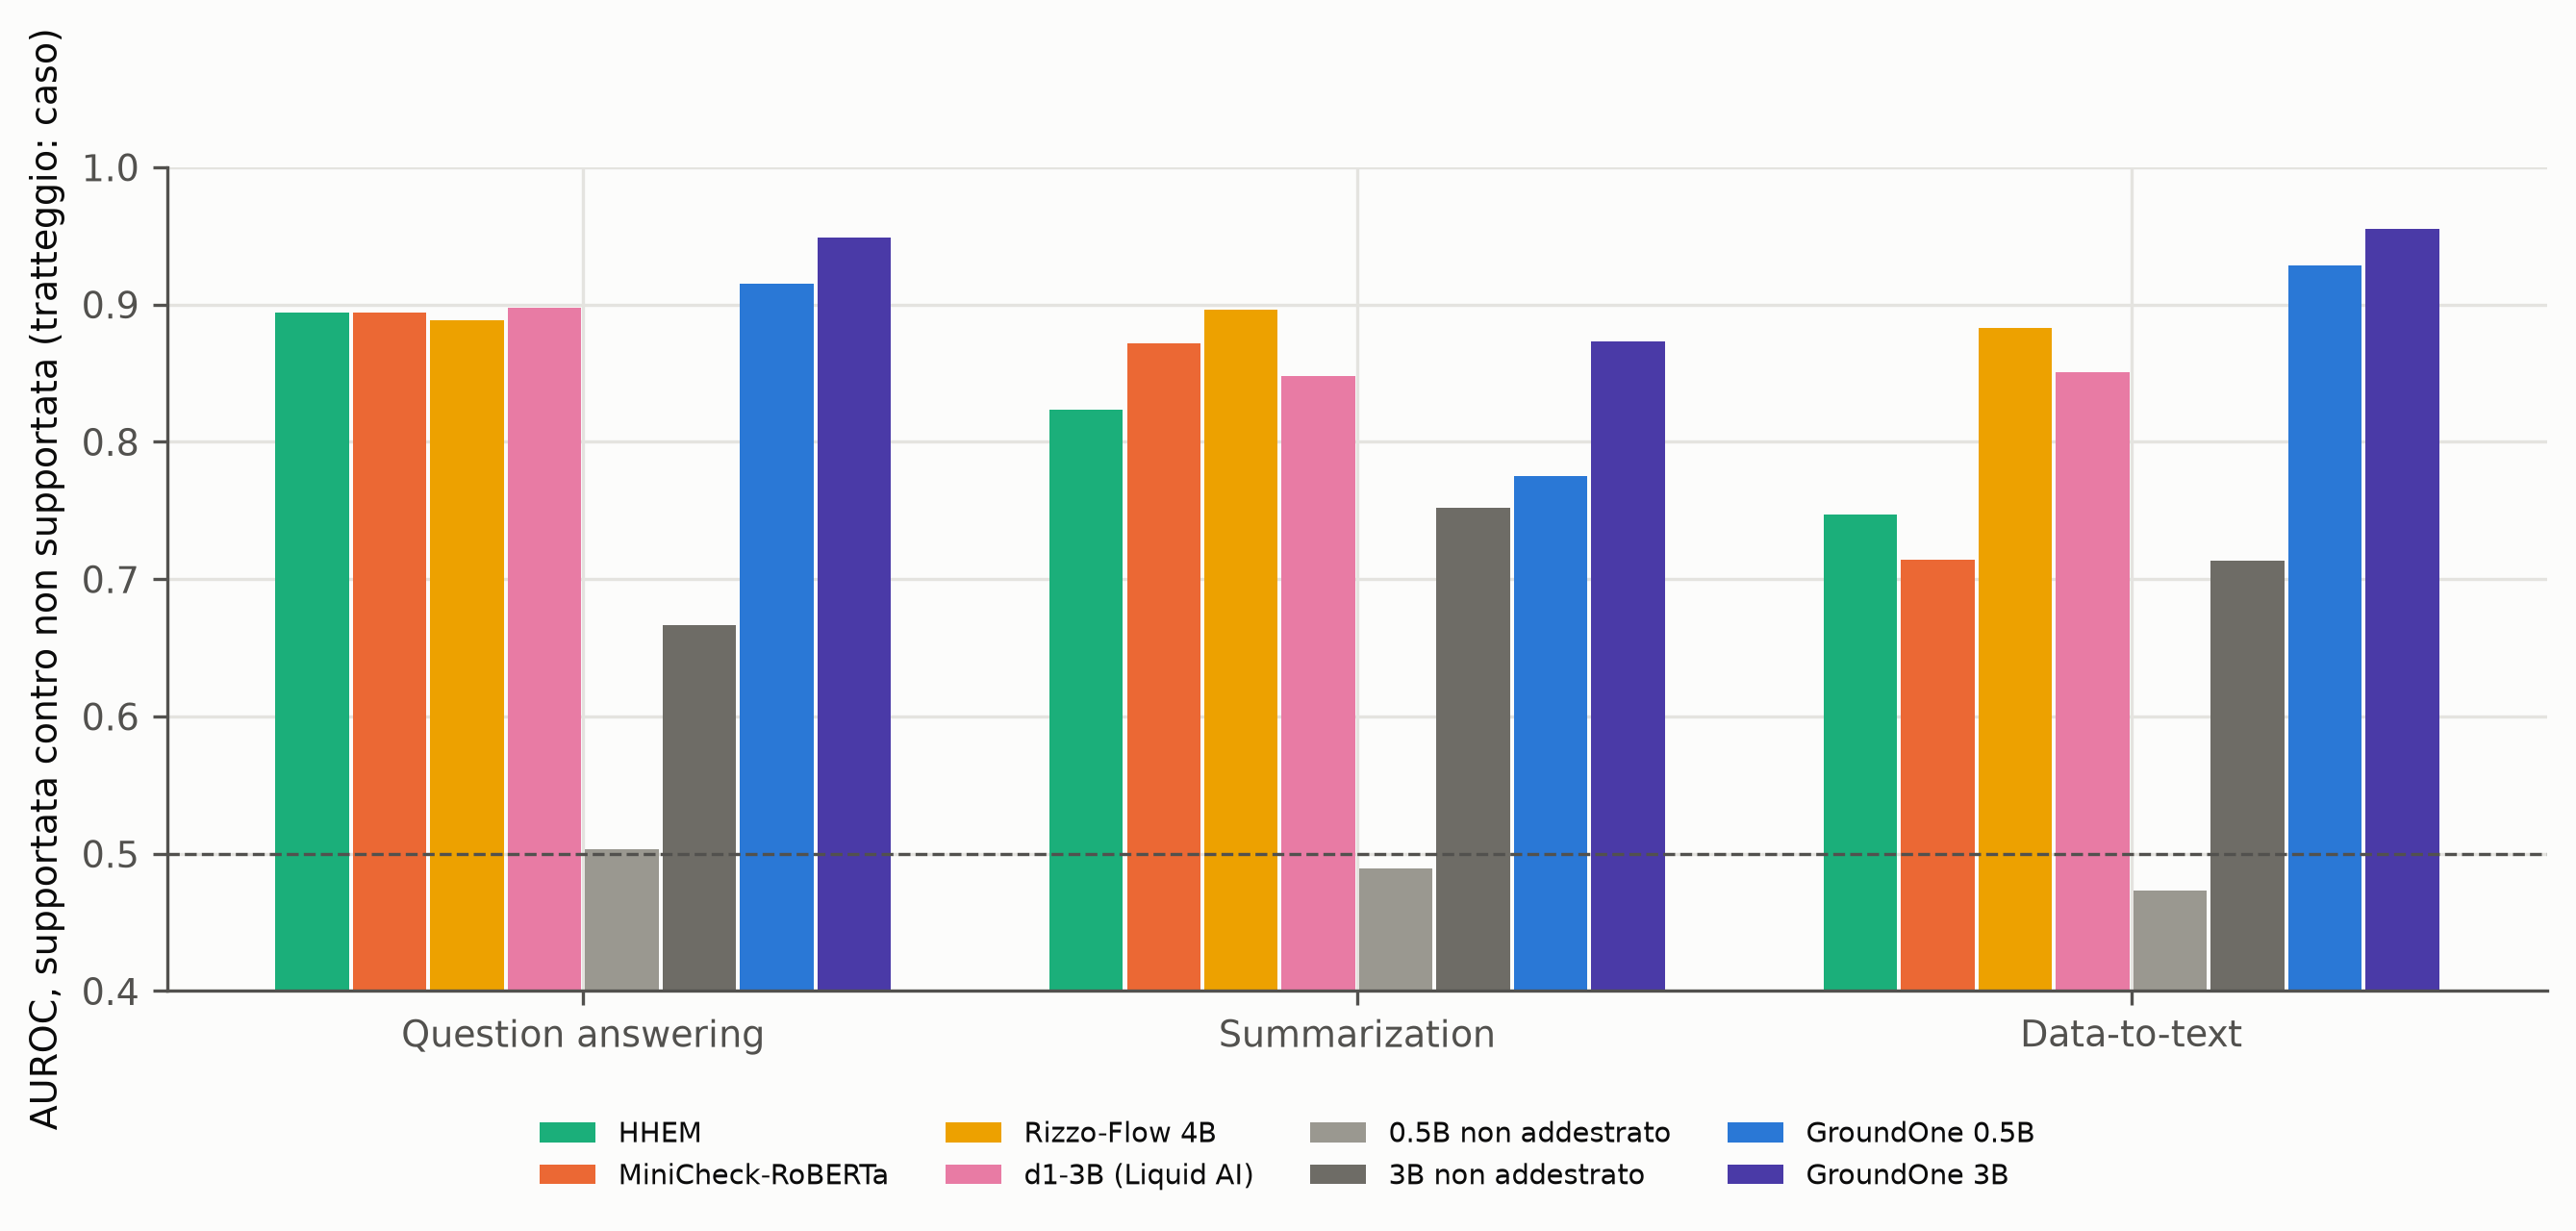
\includegraphics[width=\textwidth]{images/results/t1_by_task.png}
\caption{AUROC di $P(\text{supported})$ su T1 per task (question answering, summarization, data-to-text) e per sistema. Il vantaggio di GroundOne si concentra nel data-to-text; nella summarization MiniCheck-RoBERTa supera il 0.5B ed è alla pari con il 3B.}
\label{fig:results-by-task}
\end{figure}

I modelli non addestrati mostrano quanta parte dell'accuratezza si debba all'addestramento. Il 0.5B non addestrato è al livello casuale, con una balanced accuracy a tre classi di 0.372, perché non risponde mai ``supportata''. Il 3B non addestrato, a cui si pone la stessa domanda, raggiunge
una balanced accuracy a tre classi di 0.437, contro 0.818 dello stesso modello dopo l'addestramento, sulle stesse
risposte. Il contributo del readout ristretto, al di là dell'addestramento, è misurato separatamente nella
Sezione~\ref{sec:results-readout}.

\begin{figure}[htbp]
\centering
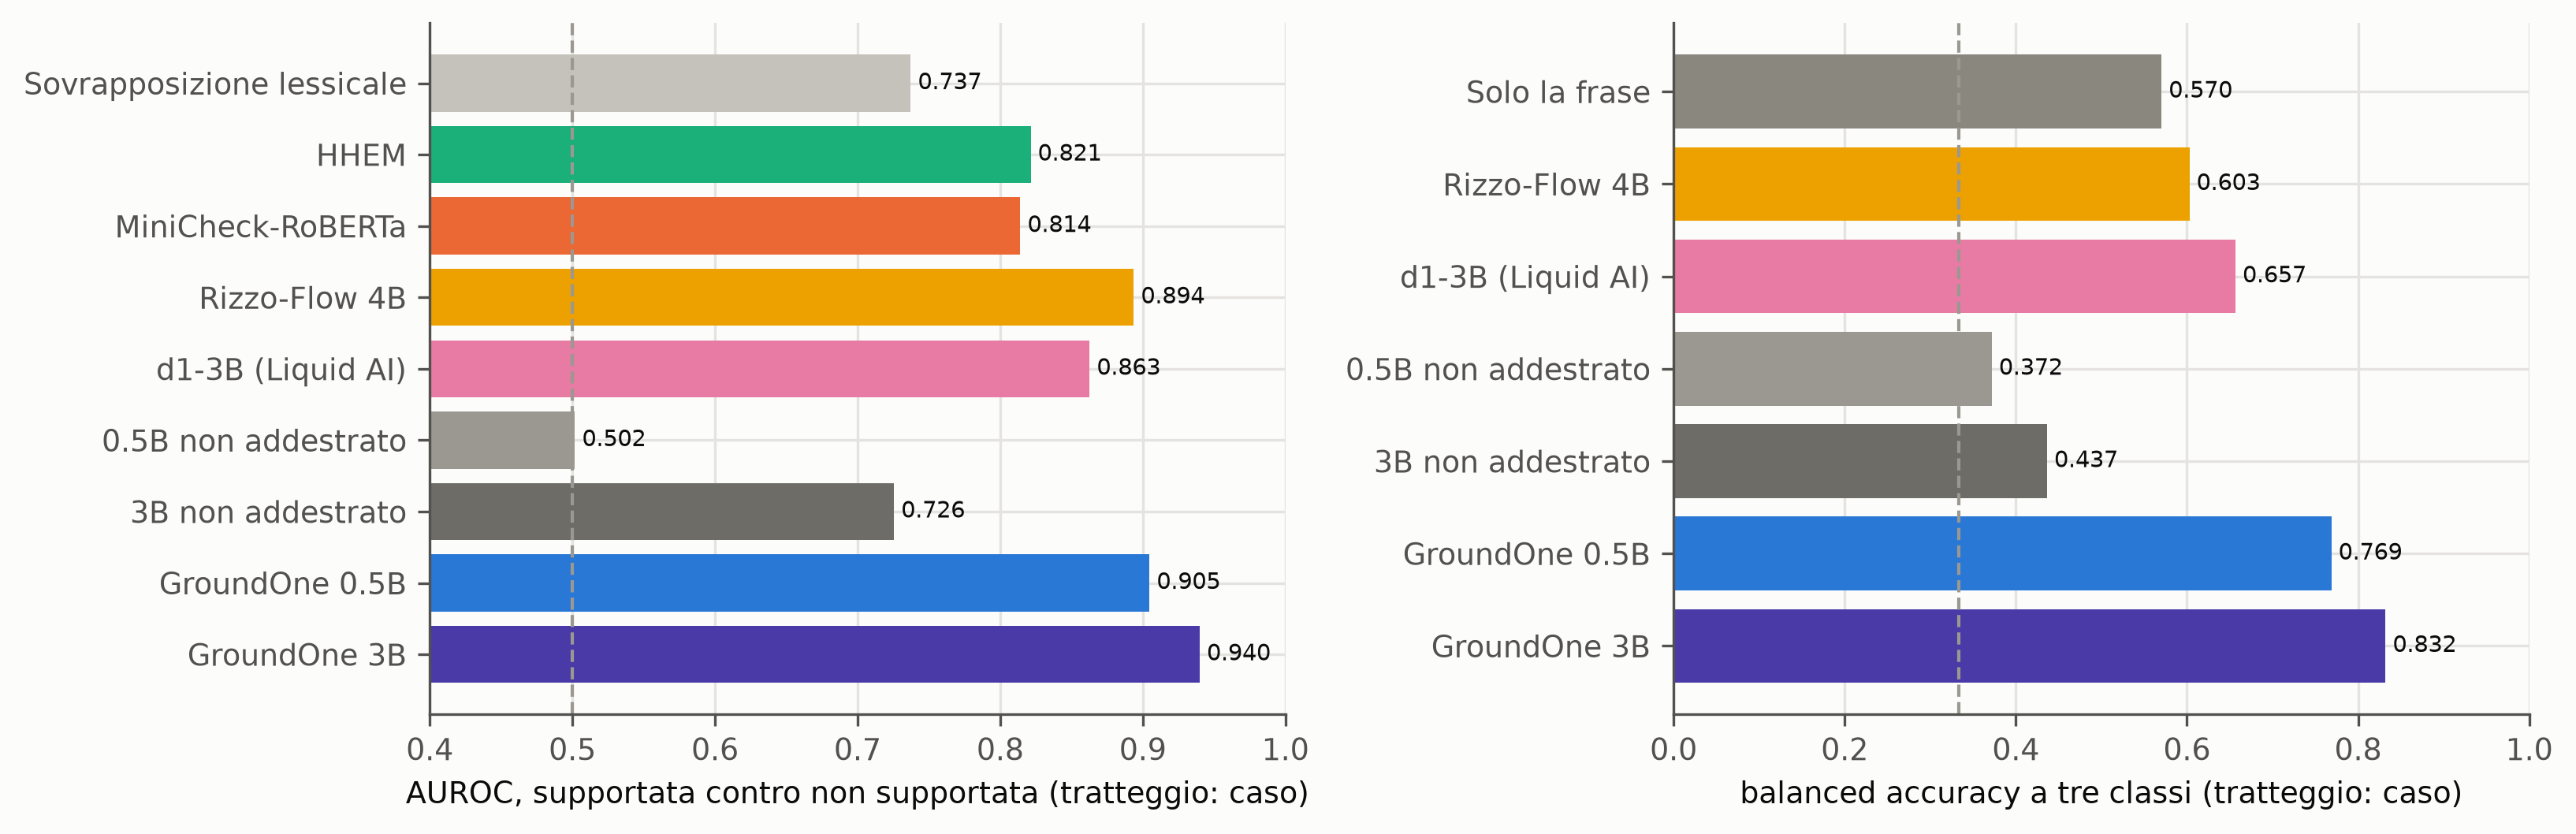
\includegraphics[width=\textwidth]{images/results/comparison_t1.png}
\caption{T1: AUROC di $P(\text{supported})$ per ogni sistema (a sinistra) e balanced accuracy a tre classi per i sistemi
che hanno un output a tre classi (a destra). Rizzo-Flow è valutato su 300 risposte e il 3B non addestrato su 600; tutti
gli altri sistemi, compreso d1-3B, sono valutati sull'intero test set.}
\label{fig:results-comparison}
\end{figure}

Il confronto più istruttivo è quello con Rizzo-Flow, il decision model generalista più grande: un modello da 4B sottoposto a
fine-tuning per decisioni generiche. Sulle stesse 300 risposte di T1, Rizzo-Flow raggiunge una balanced accuracy a tre
classi di 0.603, contro 0.798 del GroundOne 0.5B e 0.840 del 3B. Le differenze sono ampie: $+0.195$ (da $+0.140$ a $+0.251$) per il 0.5B e $+0.237$ (da $+0.184$ a $+0.289$) per il 3B. In AUROC, invece, Rizzo-Flow (0.894) è vicino al
0.5B, che su queste risposte ottiene 0.916, e la differenza non è significativa. Rizzo-Flow, infatti, ordina bene le
frasi, ma predice ``supportata'' per il 90\,\% di esse. Il 3B le ordina meglio di Rizzo-Flow ($+0.056$, da $+0.034$ a $+0.081$). Uno specialista otto volte più piccolo, quindi, supera il generalista nella decisione per cui è stato
progettato e lo eguaglia nella capacità di ordinare le frasi.

d1-3B, un decision model generalista della stessa dimensione del 3B, offre la verifica più severa del valore della
specializzazione. È infatti già addestrato a prendere decisioni tipizzate, e si differenzia da GroundOne soprattutto per
i dati su cui è stato addestrato. Sull'intero T1 raggiunge una balanced accuracy a tre classi di 0.657 e un AUROC di
0.863. Entrambi i modelli GroundOne fanno nettamente meglio. Il 0.5B, sei volte più piccolo, lo supera di $+0.112$ (da
$+0.092$ a $+0.133$) in balanced accuracy a tre classi e di $+0.042$ in AUROC; il 3B lo supera di $+0.175$ (da $+0.157$
a $+0.195$) e di $+0.077$. Il divario è massimo sulle risposte lunghe: quando la risposta contiene quattordici o più
decisioni, d1-3B scende a 0.527, mentre il GroundOne 3B resta a 0.839 ($+0.312$, da $+0.230$ a $+0.405$). Inoltre,
d1-3B riconosce soltanto metà delle frasi non menzionate (recall 0.49). Nel dominio delle risposte RAG, dunque, la
specializzazione vale molto più di un addestramento generico a prendere decisioni.

Su LLM-AggreFact (T2) il modello 0.5B raggiunge una balanced accuracy media macro di 70.1 sugli undici dataset, contro 64.2 dello stesso modello usato zero-shot (punteggio pubblicato nella leaderboard) e 72.8 del modello 7B zero-shot riportato nella leaderboard pubblica. Resta
invece 3.9 punti sotto MiniCheck-RoBERTa (74.0), una differenza significativa. Sui quattro dataset più vicini alla
retrieval-augmented generation i due sistemi sono alla pari (74.4 per GroundOne 0.5B, 74.6 per MiniCheck-RoBERTa). Nella colonna di RAGTruth GroundOne è in
vantaggio, 82.1 contro 76.5, ma il confronto lo favorisce, perché è stato addestrato sulle risposte del training set di
RAGTruth. Al di fuori del RAG, invece, il 0.5B è inferiore all'encoder di sette-nove punti su AggreFact-CNN,
AggreFact-XSum, FactCheck-GPT e REVEAL: è il costo atteso di un addestramento sui soli dati RAG.

Il modello 3B, valutato sull'intero test set, colma gran parte di questo divario. La sua balanced accuracy media macro è
74.8: è alla pari con quella di MiniCheck-RoBERTa (74.0; differenza appaiata $+0.8$ punti, intervallo da $-0.5$ a $+2.0$) e superiore al punteggio zero-shot pubblicato per il modello 7B (72.8), per il quale non si può calcolare un
intervallo. Sui dataset RAG raggiunge 76.9, 2.4 punti sopra l'encoder (intervallo da $+1.4$ a $+3.4$). Il suo guadagno
rispetto al 0.5B, $+4.7$ punti (da $+3.4$ a $+5.9$), è diffuso tra i dataset, con i miglioramenti maggiori su REVEAL,
WiCE, FactCheck-GPT e XSum: la dimensione del modello migliora quindi il trasferimento al di fuori del dominio di
addestramento. Il 3B resta nettamente sotto l'encoder soltanto nella summarization di notizie (AggreFact-CNN, 59.3
contro 67.1). Rizzo-Flow raggiunge 61.5 sui 1{,}093 elementi del suo sottocampione, e su questi elementi il GroundOne 3B
fa meglio di 12.0 punti (da $+7.6$ a $+16.4$).

Su questo benchmark, tuttavia, i sistemi più forti restano sopra GroundOne. Una valutazione indipendente del decision model
closed Jev, sullo stesso test set e con la stessa metrica, riporta 78.6, e 76.9 per un modello open da 27B letto
attraverso le lettere di risposta. I prompt sono diversi da quelli usati qui, e non è possibile calcolare alcun
intervallo~\cite{deusser2026jev}. Su un benchmark ampio di groundedness, quindi, uno specialista da 3B addestrato
soltanto su risposte RAG eguaglia il miglior encoder di piccole dimensioni, ma resta sotto lo stato dell'arte closed e
sotto modelli open molto più grandi. Il generalista d1-3B conferma il quadro quando la dimensione è la stessa. Su un
sottocampione casuale di 4{,}000 elementi raggiunge 75.7, contro 74.3 del GroundOne 3B sugli stessi elementi, una
differenza non significativa ($-1.3$, da $-4.0$ a $+1.0$), mentre supera il 0.5B di 6.5 punti. Rispetto al GroundOne
3B, d1-3B è più debole nella colonna di RAGTruth (78.9 contro 87.3) e nettamente più forte su WiCE e sulla summarization
di dialoghi.

\section{Trasferimento a un dominio diverso (T3)}
\label{sec:results-t3}

Su VitaminC il quadro si rovescia. Sull'intero test set il 0.5B raggiunge una balanced accuracy a tre classi di 0.442 e
il 3B di 0.527, con un AUROC rispettivamente di 0.722 e di 0.817, mentre MiniCheck-RoBERTa arriva a un AUROC di 0.968.
Sulle 600 coppie valutate con Rizzo-Flow, il modello generalista ottiene una balanced accuracy a tre classi di 0.712 e un
AUROC di 0.909, contro 0.442 e 0.744 del 0.5B e 0.537 e 0.845 del 3B. La Figura~\ref{fig:results-comparison-t3} mostra il confronto completo su T3.

\begin{figure}[htbp]
\centering
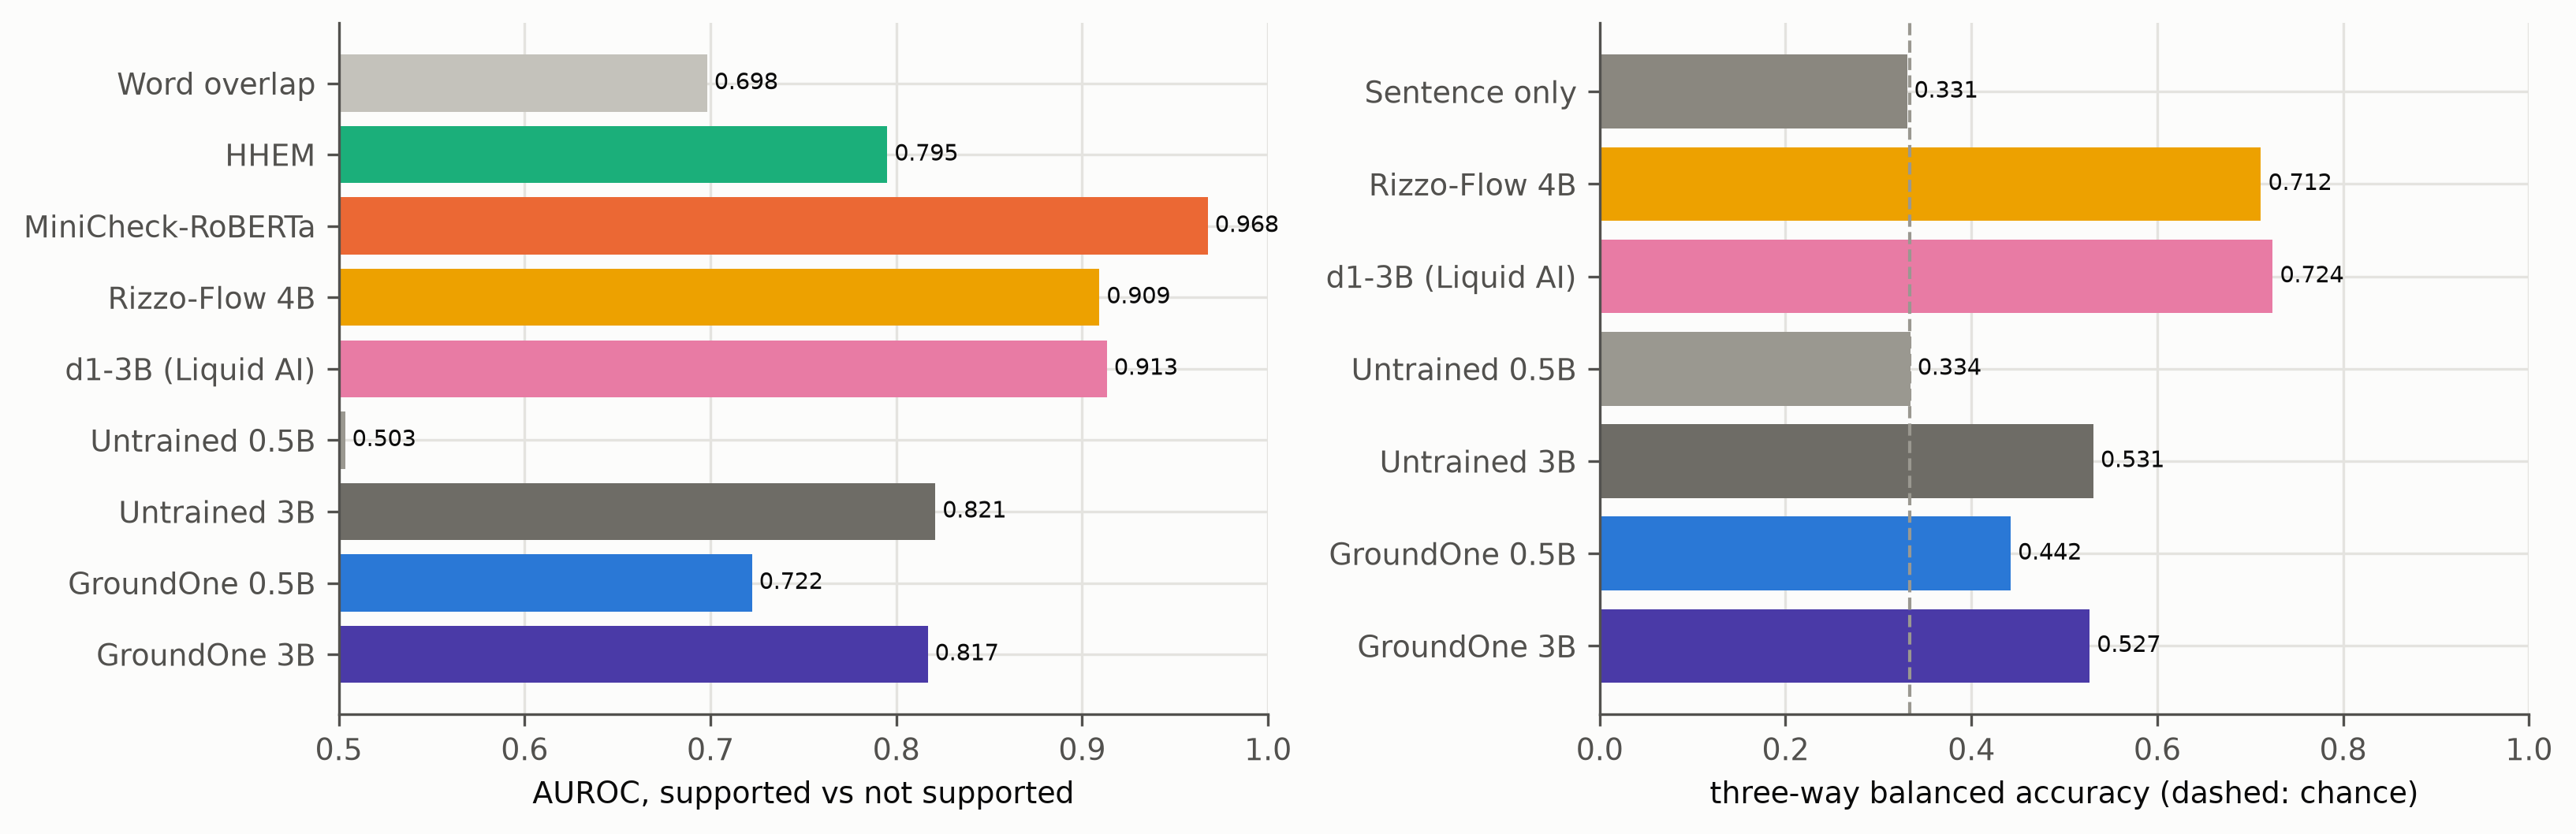
\includegraphics[width=\textwidth]{images/results/comparison_t3.png}
\caption{Confronto dei sistemi su T3 (VitaminC): a sinistra l'AUROC di $P(\text{supported})$, a destra la balanced accuracy a tre classi per i sistemi con un output a tre classi. Rizzo-Flow è valutato su un sottocampione di 600 coppie; il tratteggio indica il livello casuale. Per MiniCheck-RoBERTa VitaminC fa parte della genealogia dei dati di addestramento.}
\label{fig:results-comparison-t3}
\end{figure}

Due fatti aiutano a interpretare questi numeri. Il primo è che MiniCheck-RoBERTa parte dal modello AlignScore, i cui
dati di addestramento comprendono VitaminC~\cite{zha2023alignscore}. Per l'encoder, quindi, T3 appartiene alla
distribuzione di addestramento, mentre per GroundOne misura il trasferimento da RAGTruth. Il secondo è che il guadagno
del 3B sul 0.5B in T3 si deve alla dimensione del modello più che all'addestramento su dati RAG: il 3B non addestrato
raggiunge già 0.531 e un AUROC di 0.821. d1-3B, il decision model generalista della stessa dimensione, rende esplicito il
contrasto. Sull'intero T3 raggiunge 0.724 e un AUROC di 0.913, e supera il GroundOne 3B di 0.197 e di 0.096: l'esatto
opposto di quanto accade su T1. La specializzazione su risposte RAG migliora quindi in modo sostanziale il task RAG, ma
da sola non basta a produrre un fact checker generale. La Sezione~\ref{sec:results-errors} mostra quali casi sfuggono.

\section{Readout e generazione a confronto}
\label{sec:results-readout}

Il controllo B2 isola il contributo del readout. Il confronto mantiene invariati i pesi ottenuti con il fine-tuning, il
prompt e il singolo forward pass, e cambia soltanto il modo in cui si ricava il verdetto a ogni marker. Il verdetto è
letto dalle tre lettere di risposta, come fa GroundOne, oppure è il token che emetterebbe la generazione greedy
(Figura~\ref{fig:results-readout}). Per il 0.5B il token generato dà una balanced accuracy a tre classi di 0.521, contro
0.769 del readout, con una differenza di $+0.248$ (da $+0.228$ a $+0.268$) a favore del readout. In un quarto dei marker
(24.7\,\%) il modello non emetterebbe affatto una lettera, ma per lo più un semplice spazio, cioè l'inizio di una risposta
più lunga. Per il 3B, invece, il token generato è quasi sempre una lettera (1.2\,\% di errori di formato) e concorda con
il readout nel 92\,\% dei marker; eppure il readout resta migliore, con 0.832 contro 0.761 ($+0.071$, da $+0.059$ a $+0.082$). Quando la risposta contiene quattordici o più decisioni, il divario è massimo per il modello piccolo: $+0.346$.

\begin{figure}[htbp]
\centering
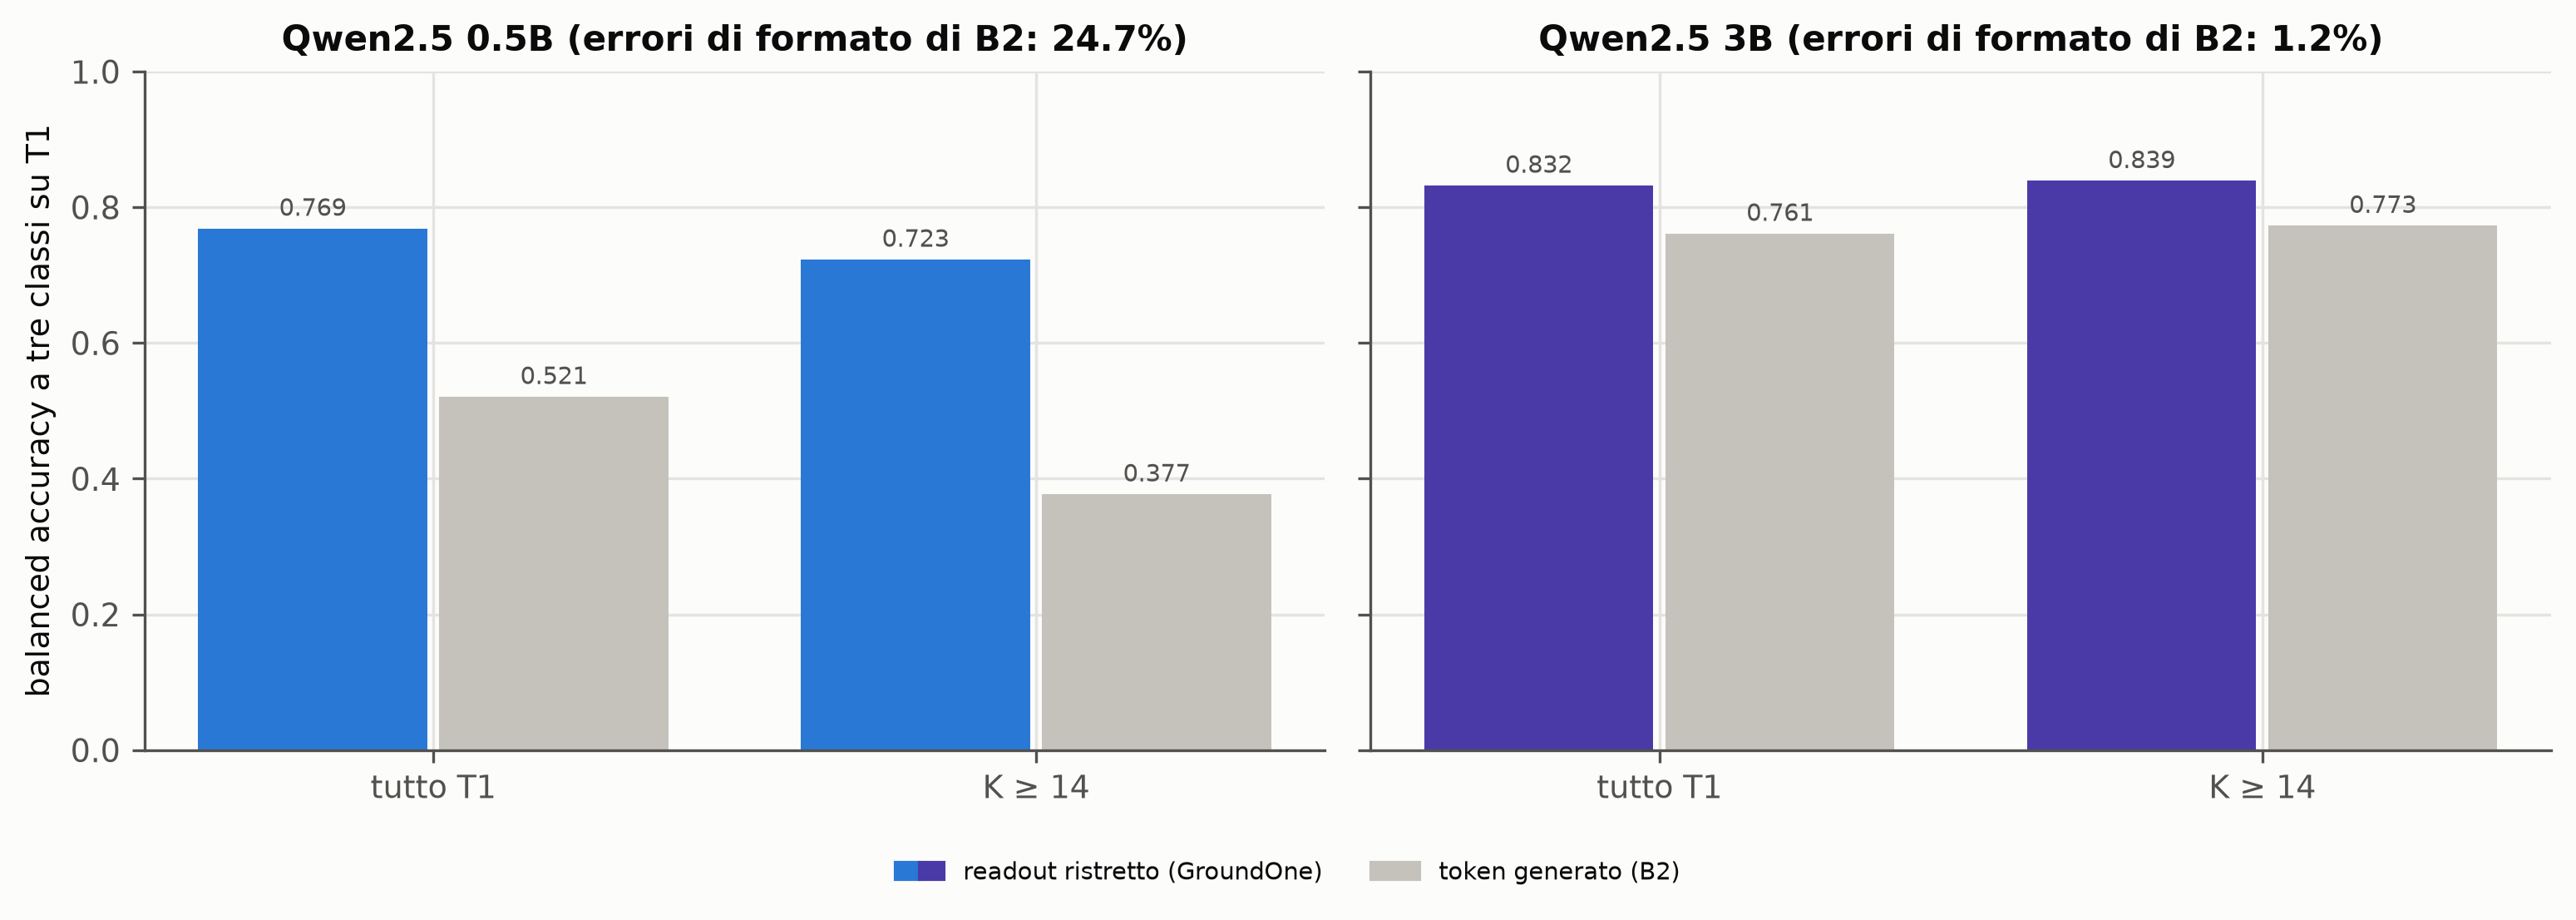
\includegraphics[width=\textwidth]{images/results/readout_vs_generation.png}
\caption{Controllo B2 sull'intero T1. Con gli stessi pesi e lo stesso forward pass, il verdetto è letto dalle tre lettere
di risposta (GroundOne) oppure preso come il token che emetterebbe la generazione greedy; gli errori di formato sono
contati come errori.}
\label{fig:results-readout}
\end{figure}

Le due opzioni hanno la stessa latenza, perché entrambe richiedono un solo forward pass: a cambiare è soltanto la regola
di decisione. Restringere la scelta alle opzioni ammissibili elimina per costruzione gli errori di formato. Inoltre,
poiché il modello è addestrato soltanto a ordinare le tre lettere, la scelta ristretta fornisce anche la decisione più
accurata (Sezione~\ref{sec:method-readout}). Questa restrizione conta tanto più quanto più il modello è piccolo. Si
ripete spesso che leggere i logit delle risposte e generare un singolo token di risposta siano operazioni equivalenti:
per un verificatore sottoposto a fine-tuning l'equivalenza vale per il costo, ma non per l'accuratezza.

\section{Calibrazione e selective prediction}
\label{sec:results-calibration}

Prima della calibrazione, le probabilità sottostimano il supporto. Nel reliability diagram
(Figura~\ref{fig:results-reliability}) la curva delle probabilità grezze giace sopra la diagonale, perché i pesi delle
classi addestrano il modello come se le classi fossero bilanciate. L'ECE binario su T1 è 0.30 per il 0.5B e 0.18 per il
3B. La temperatura e il bias stimati sul dev set lo portano a 0.019 per entrambi i modelli, e a 0.020 per la seconda
esecuzione del 0.5B. Riducono inoltre la negative log-likelihood da 0.55 a 0.21 per il 0.5B e da 0.36 a 0.17 per il 3B,
lasciando l'AUROC praticamente invariato. La mappa stimata sul dev set si trasferisce quindi al test set dello stesso
dominio. La Figura~\ref{fig:results-reliability-3b} mostra lo stesso diagramma per il 3B.

\begin{figure}[htbp]
\centering
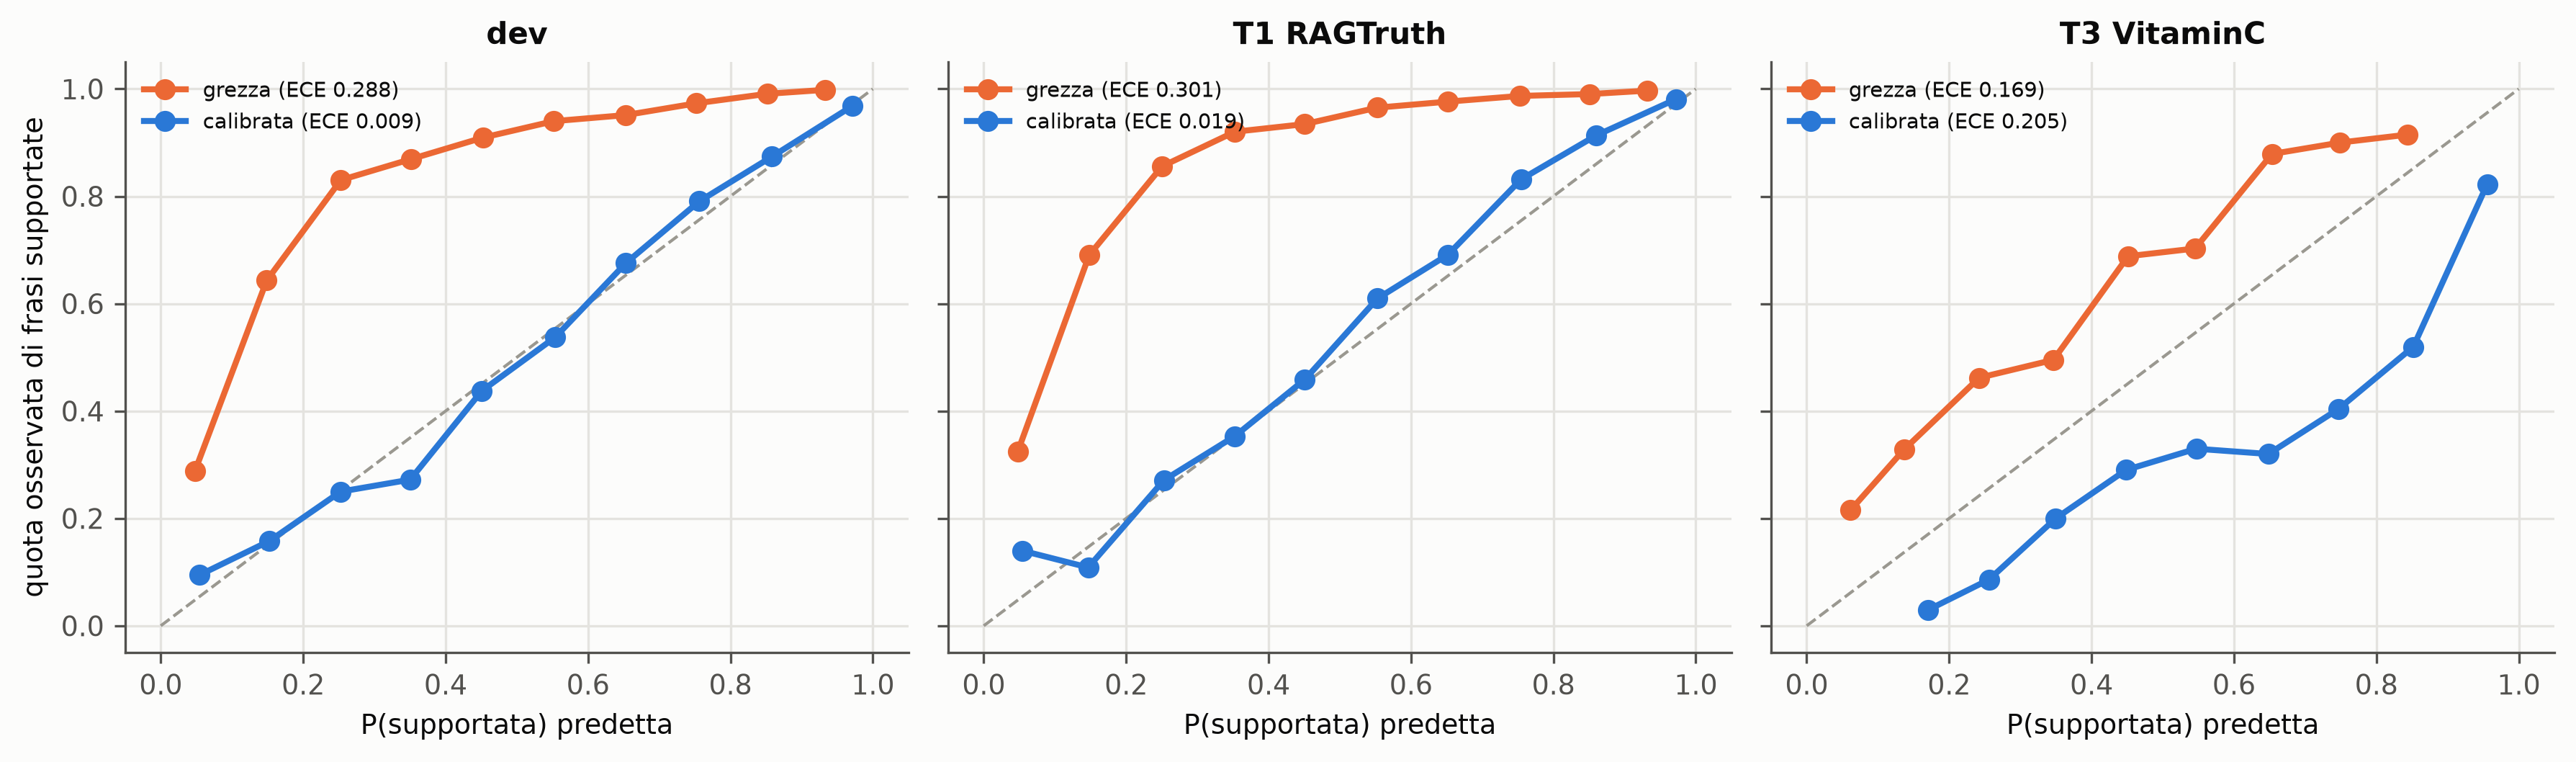
\includegraphics[width=\textwidth]{images/results/g1-05b-reliability.png}
\caption{Reliability diagram di $P(\text{supported})$ del 0.5B, prima della calibrazione (grezza) e dopo la calibrazione
stimata sul dev set, per il dev set, T1 e T3. Ogni punto rappresenta una fascia di probabilità che contiene almeno 20
frasi.}
\label{fig:results-reliability}
\end{figure}

\begin{figure}[htbp]
\centering
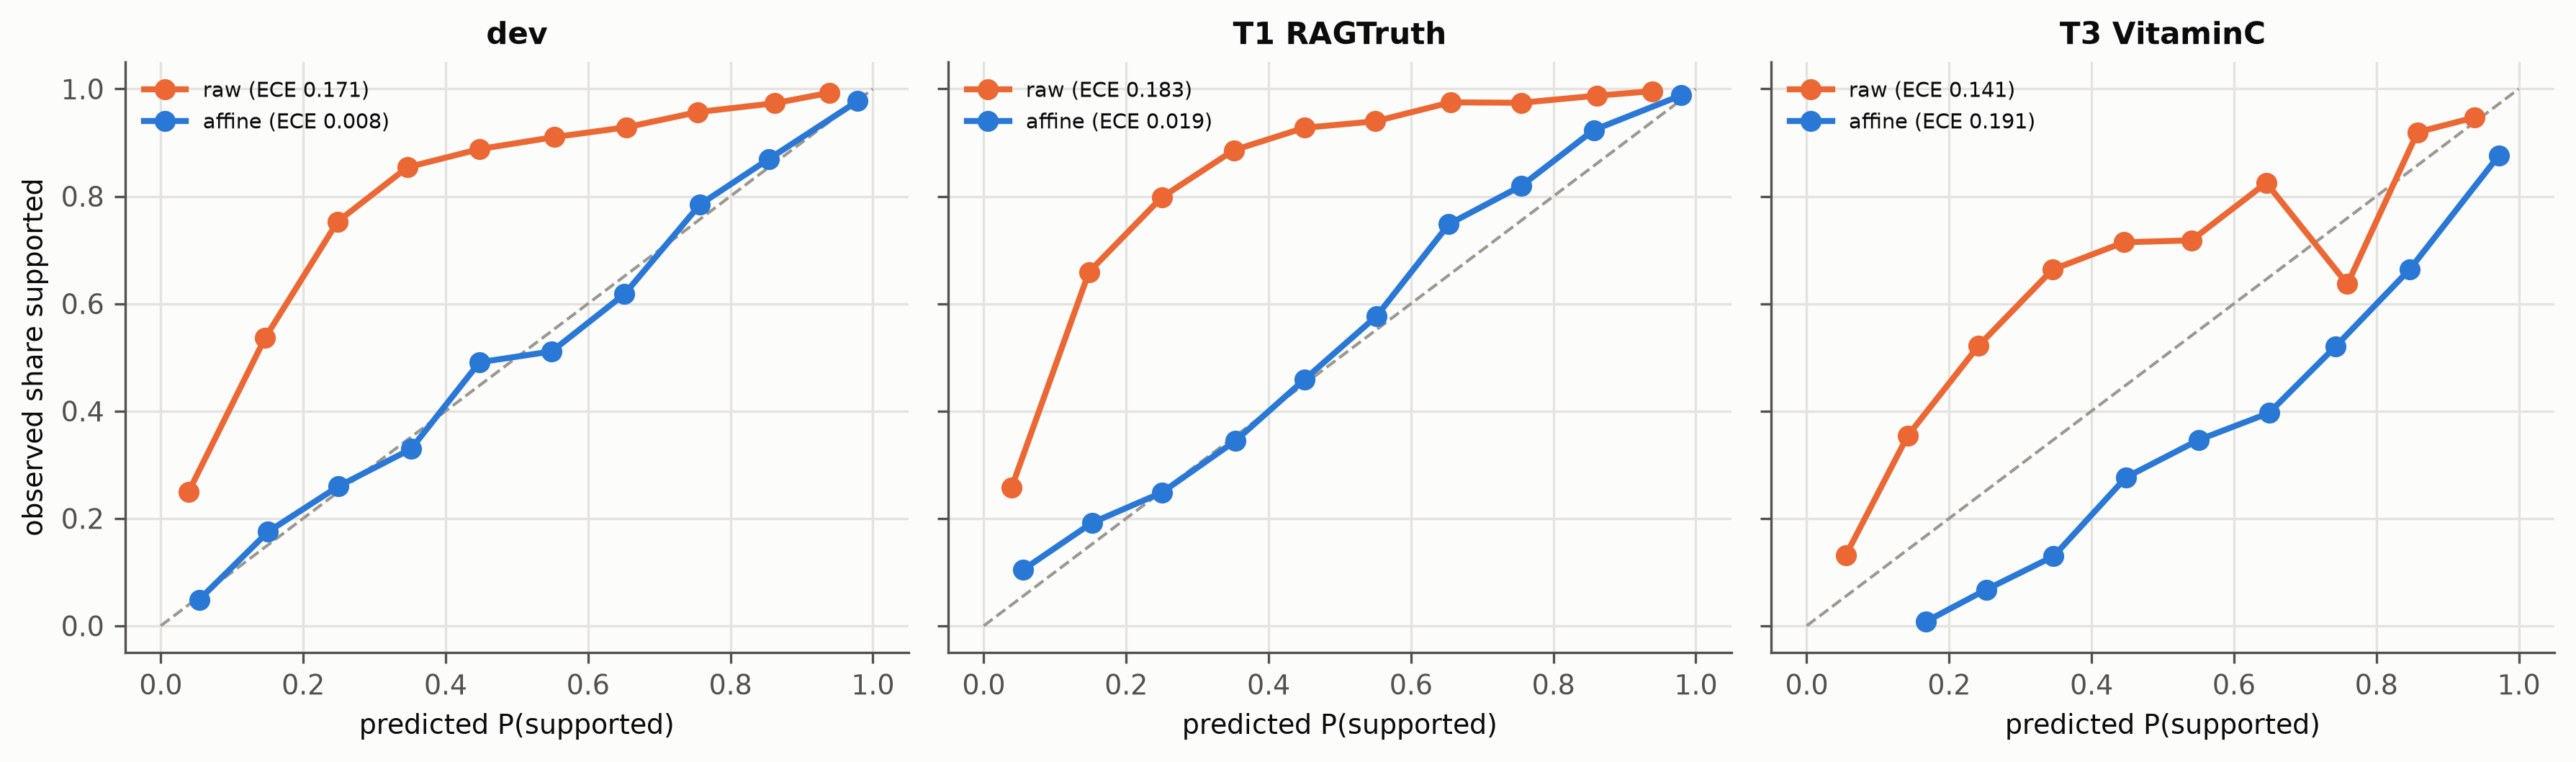
\includegraphics[width=\textwidth]{images/results/g1-3b-reliability.png}
\caption{Reliability diagram di $P(\text{supported})$ del 3B, prima e dopo la calibrazione stimata sul dev set, per il dev set, T1 e T3; ogni punto è una fascia di probabilità con almeno 20 frasi. Come per il 0.5B, la calibrazione si trasferisce a T1 ma non a T3.}
\label{fig:results-reliability-3b}
\end{figure}

La calibrazione ha però una conseguenza da tenere presente. Il bias ripristina la frequenza reale di ciascuna classe,
per cui la classe più probabile dopo la calibrazione diventa più spesso ``supportata''. Per il 0.5B su T1 l'accuratezza
sale così da 0.82 a 0.93, ma la balanced accuracy a tre classi scende da 0.77 a 0.63. Quando i tre tipi di errore hanno
lo stesso peso, quindi, scegliere la classe calibrata più probabile non è una buona regola di decisione. La regola con
cui vengono restituite le etichette, descritta nella Sezione~\ref{sec:method-calibration}, risolve il problema. La regola
usa una soglia $\tau$ stimata sul dev set, pari a 0.935 per il 0.5B, a 0.895 per la sua seconda esecuzione e a 0.925 per
il 3B. Con queste soglie raggiunge su T1 una balanced accuracy a tre classi di 0.758, 0.769 e 0.830, entro circa 0.01 dalla decisione grezza valutata in tutto il capitolo, e mantiene le etichette coerenti con le probabilità calibrate. Le soglie sono alte perché circa l'88\,\% delle frasi di addestramento e del dev set è supportato: una frase viene restituita come supportata soltanto
quando il modello è molto sicuro.

Usate come confidenze, le probabilità calibrate rendono efficace la selective prediction. Rinviare le frasi su cui il
modello è meno sicuro riduce rapidamente il tasso di errore della decisione binaria: su T1 l'AURC è 0.015 per il 0.5B e 0.010 per il 3B (Figura~\ref{fig:results-risk}).

\begin{figure}[htbp]
\centering
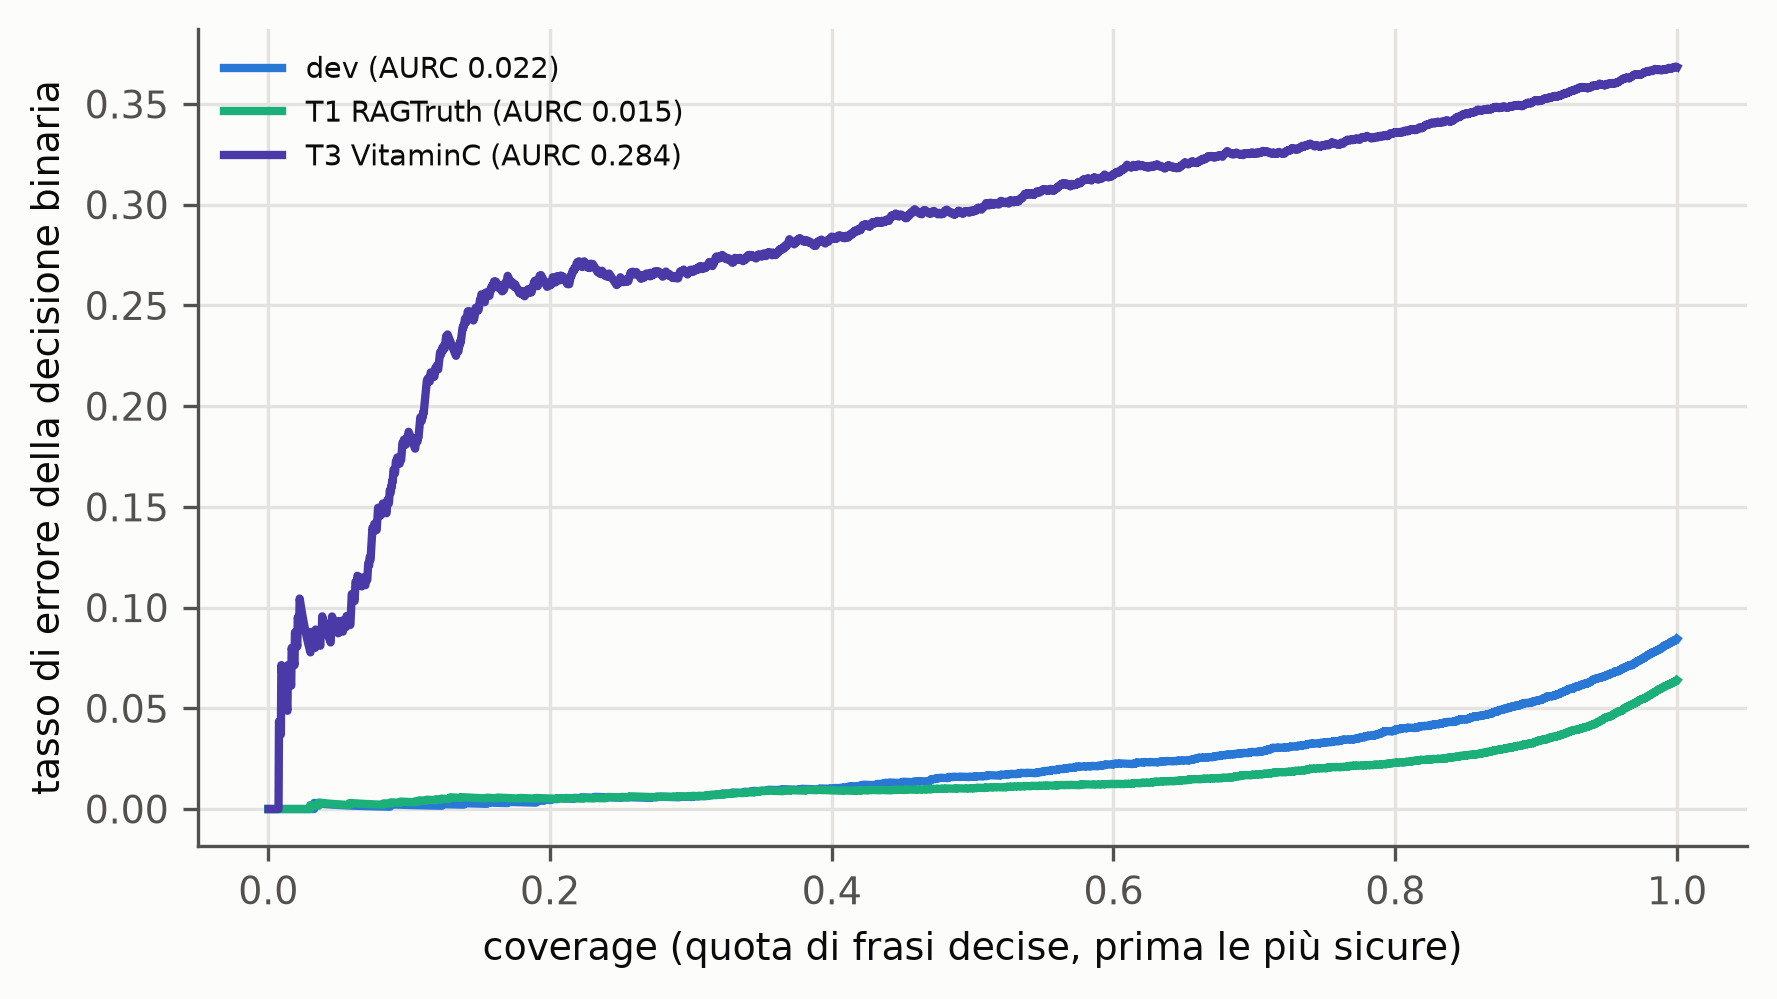
\includegraphics[width=0.75\textwidth]{images/results/g1-05b-risk_coverage.png}
\caption{Curve risk--coverage della decisione binaria del 0.5B con probabilità calibrate: tasso di errore al crescere
del numero di frasi meno sicure che vengono rinviate.}
\label{fig:results-risk}
\end{figure}

Su VitaminC, invece, la calibrazione non si trasferisce. L'ECE binario sale da 0.17 a 0.21 per il 0.5B e da 0.14 a 0.19
per il 3B, e la regola di restituzione delle etichette perde 0.02--0.04 rispetto alla decisione grezza. Il bias, infatti,
codifica il tasso di base di RAGTruth, mentre VitaminC è bilanciato per costruzione. Una calibrazione vale per la
distribuzione su cui è stata stimata, per cui ogni impiego reale richiede un piccolo campione etichettato dei propri
dati.

\section{Probabilità a parità di output}
\label{sec:results-equal-output}

I giudici LLM a parità di output servono a stabilire se un giudice LLM della stessa dimensione, a cui si chiede lo
stesso contenuto di GroundOne, possa eguagliare la qualità delle sue probabilità. La risposta è negativa
(Figura~\ref{fig:results-equal}). Il confronto usa le 200 risposte del sottoinsieme di latenza, con tutti i sistemi
calibrati allo stesso modo sul dev set. Per il 0.5B e per il 3B rispettivamente, l'AUROC di $P(\text{supported})$ è 0.94
e 0.97 per GroundOne, 0.48 e 0.68 per il giudice LLM le cui probabilità sono lette dai logit, e 0.47 e 0.58 per il giudice LLM
che le scrive. L'AURC è 0.009 e 0.005 per GroundOne, contro valori da 0.048 a 0.063 per i
giudici LLM, cioè da circa sette a dodici volte maggiori di quelli di GroundOne della stessa dimensione. L'accuratezza delle decisioni segue lo stesso andamento: 0.835 e 0.900
per GroundOne, al massimo 0.41 per qualsiasi giudice LLM.

\begin{figure}[htbp]
\centering
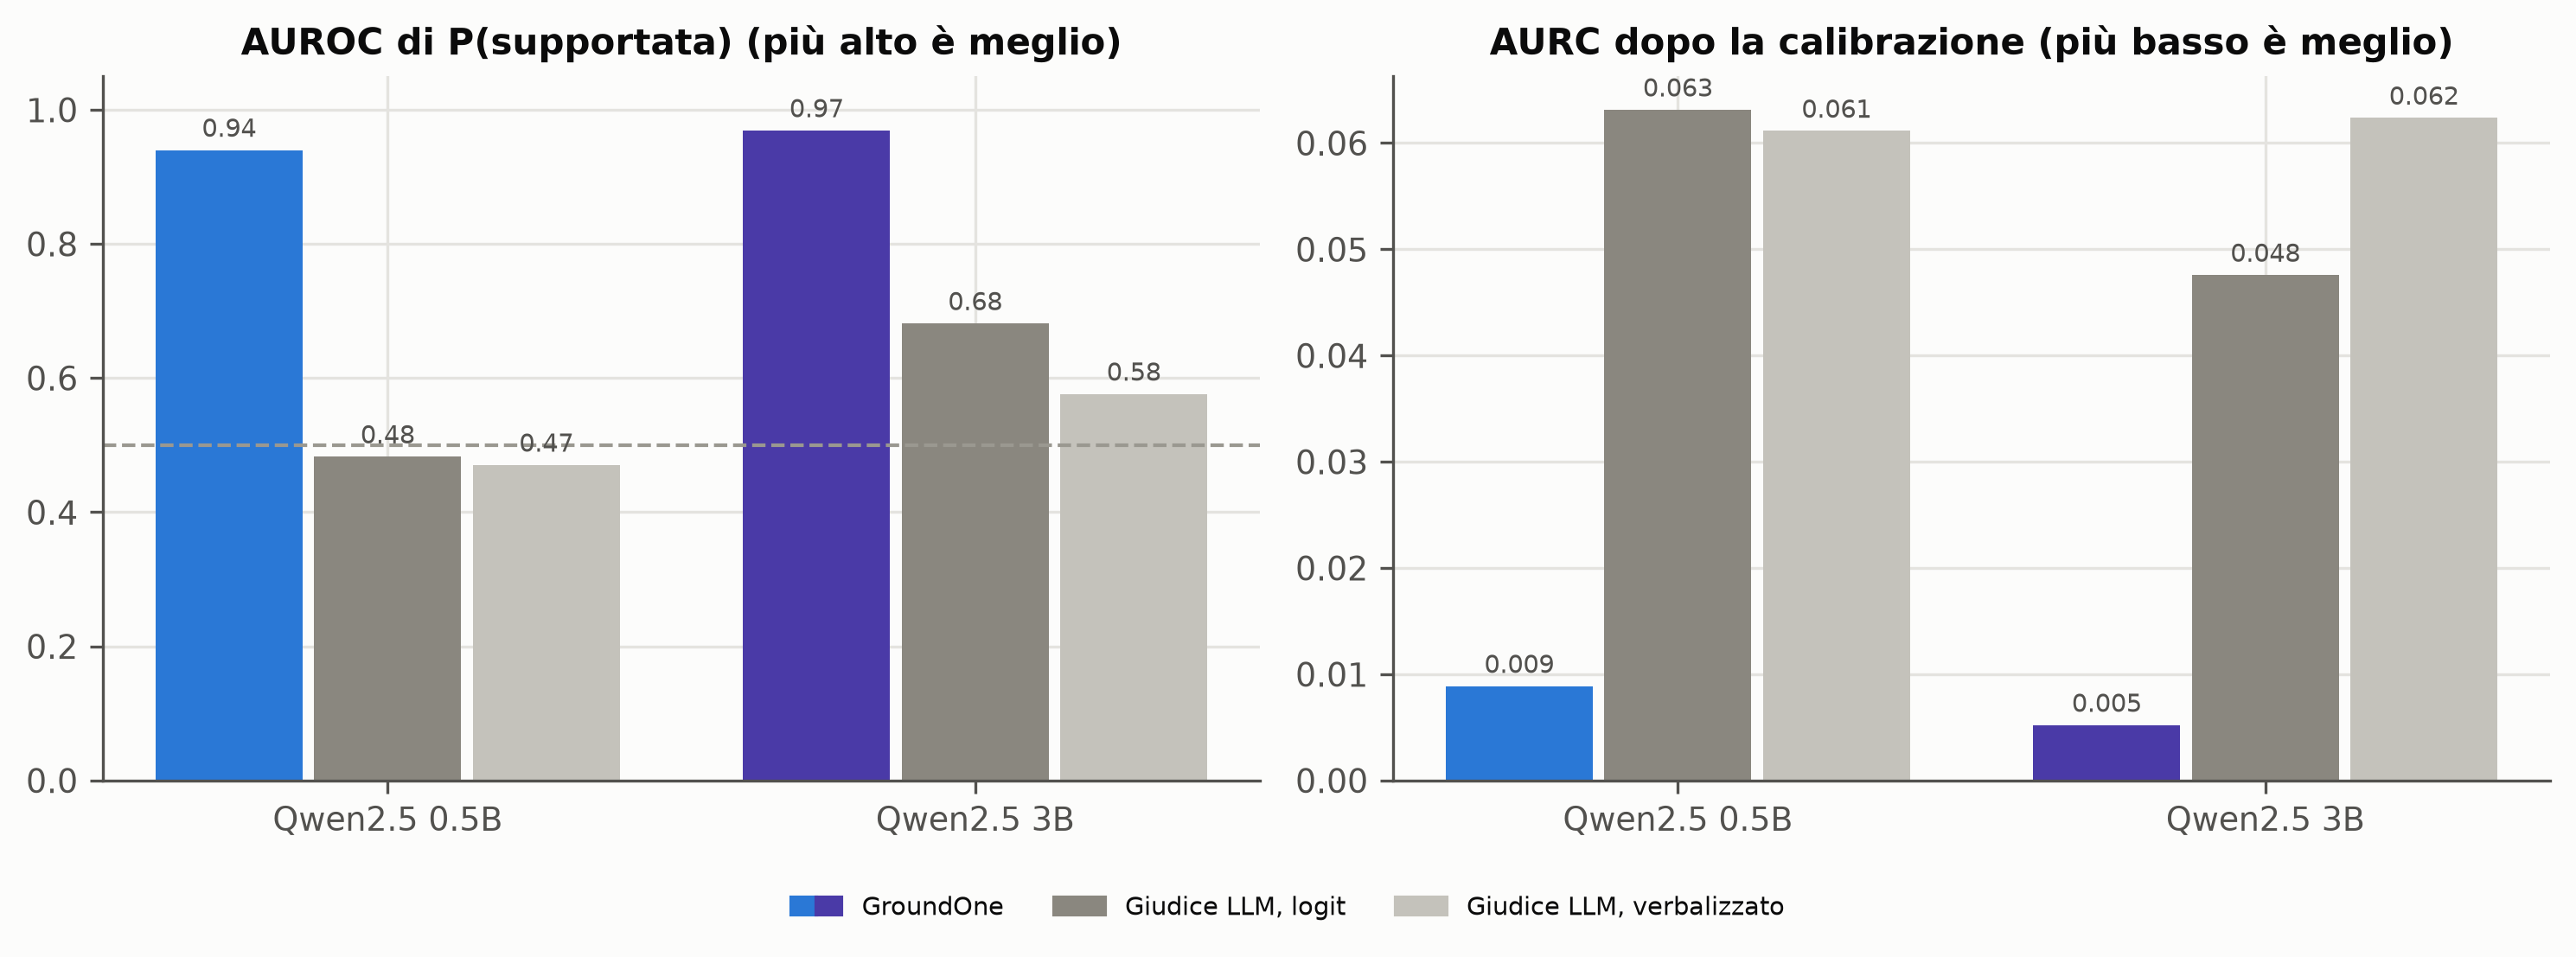
\includegraphics[width=\textwidth]{images/results/equal_output_judges.png}
\caption{Confronto a parità di output sulle 200 risposte del sottoinsieme di latenza. Ai giudici LLM della stessa
dimensione si chiede l'output di GroundOne, con le probabilità lette dai logit della lettera generata oppure scritte in
JSON; tutti i sistemi sono calibrati sul dev set con la stessa mappa. Sono considerate soltanto le frasi con un verdetto
valido.}
\label{fig:results-equal}
\end{figure}

Nella pratica contano altre due osservazioni. La prima è che le probabilità scritte a parole non portano quasi alcuna
informazione. Il 3B scrive un vettore con tutta la massa su una sola classe per il 93\,\% delle frasi, e usa appena
sedici vettori distinti. Il 0.5B scrive invece pareggi non informativi, come probabilità uguali per tutte le classi: se
i pareggi privi di etichetta vengono contati come errori, la sua balanced accuracy scende da 0.234 a 0.081. Il dato
concorda con l'osservazione che la confidenza verbalizzata dei modelli piccoli è grossolana e poco
informativa~\cite{xiong2024uncertainty,tian2023justask}. La seconda osservazione è che l'ECE, da solo, nasconderebbe
tutto ciò. Dopo la calibrazione ogni sistema, giudici LLM compresi, ottiene un ECE binario compreso tra 0.03 e 0.05, perché
una mappa di calibrazione può allineare la confidenza media al tasso di base anche quando le probabilità non separano le
classi. La capacità discriminativa va quindi misurata a parte, con l'AUROC e con l'AURC.

Chiedere le probabilità, infine, ha un costo. Il giudice LLM che le legge dai logit è veloce quanto il giudice LLM sintetico,
perché genera le stesse lettere. Il giudice LLM che scrive l'oggetto JSON, invece, impiega con il 3B 17.0 secondi per una
risposta con quattordici o più decisioni, quanto il giudice LLM verboso, e non è più accurato del giudice LLM sintetico.

\section{Latenza in funzione di $K$}
\label{sec:results-latency}

La Figura~\ref{fig:results-latency} riporta la misura centrale della tesi: il tempo necessario per verificare una
risposta al crescere del numero di decisioni, misurato sulle stesse 200 risposte di T1. Tra i sistemi eseguiti
in-process su MLX, GroundOne è il più veloce con entrambe le dimensioni e in ogni fascia di $K$, e il suo vantaggio
aumenta con $K$. Quando la risposta contiene quattordici o più decisioni, il GroundOne 0.5B impiega 0.41 secondi, contro
0.80 del giudice LLM sintetico e 2.51 del giudice LLM verboso della stessa dimensione. È quindi 1.95 volte più veloce del primo
(da 1.82 a 2.12) e 6.16 volte più veloce del secondo (da 5.72 a 6.66). Nella stessa fascia il GroundOne 3B impiega 2.57
secondi, contro 4.44 e 15.86 secondi dei due giudici LLM 3B, ed è quindi 1.73 volte (da 1.65 a 1.82) e 6.18 volte (da 5.88 a 6.63) più veloce.

Leggere tutti i verdetti in un unico forward pass è anche più rapido che porre una domanda per frase in un batch: ai
valori più alti di $K$ il guadagno è di un fattore 1.4--1.5. L'altra leva è la dimensione del modello: il GroundOne 0.5B
verifica una risposta circa sei volte più in fretta del 3B, con un tempo mediano di 0.33 secondi contro 1.99.

\begin{figure}[htbp]
\centering
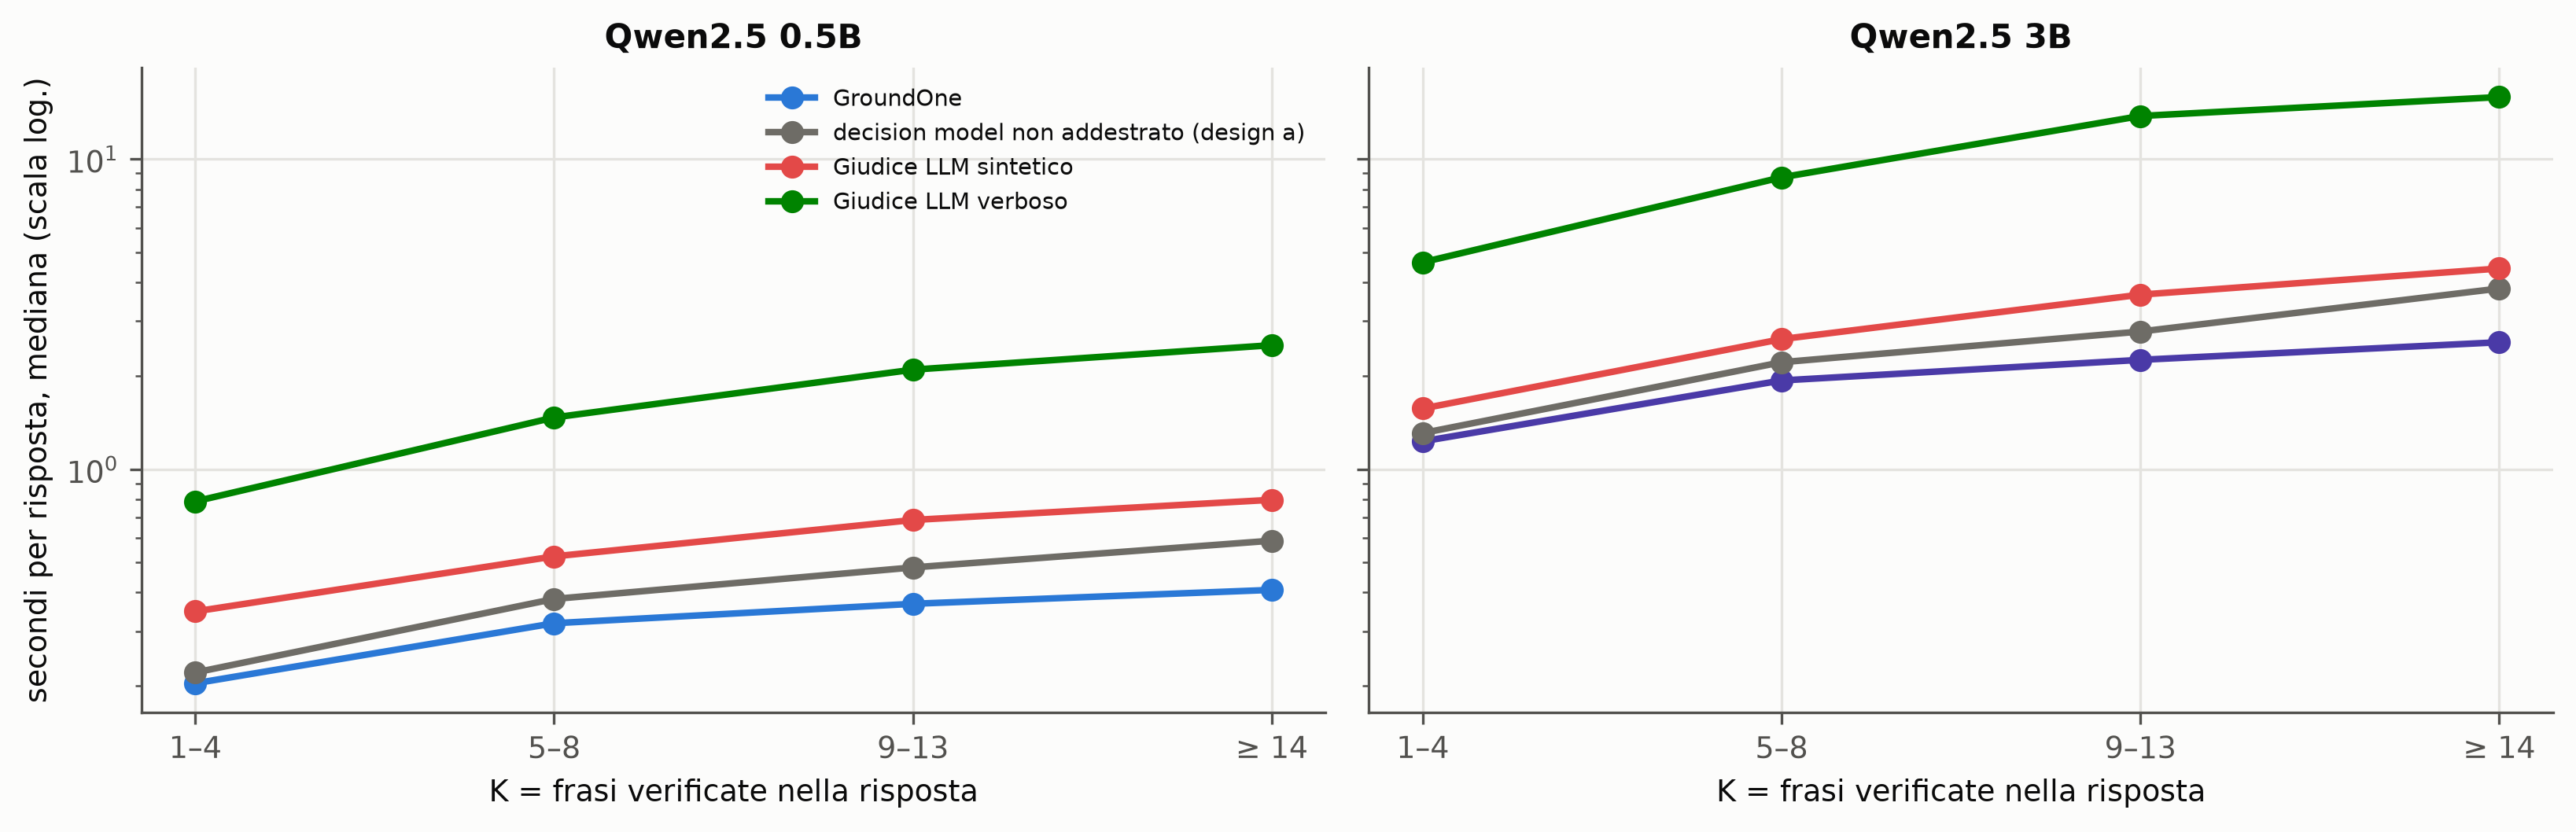
\includegraphics[width=\textwidth]{images/results/latency_vs_K.png}
\caption{Tempo mediano per risposta in funzione di $K$ sulle stesse 200 risposte di T1 (MLX in-process, una risposta
alla volta, M4 con 16\,GB). Sono confrontati GroundOne, il decision model con una domanda per frase e i giudici LLM
sintetico e verboso. Scala logaritmica.}
\label{fig:results-latency}
\end{figure}

\subsection{Lettura del testo e decisione}
\label{sec:results-latency-split}

Il tempo di GroundOne cresce con $K$, ma non per il numero di decisioni in sé. Le risposte con più frasi sono anche più
lunghe: nel sottoinsieme di latenza il prompt passa da circa 550 token nella fascia $K \leq 4$ a circa 1{,}140 token
con $K \geq 14$, e il tempo del prefill cresce con la lunghezza del testo. Per separare le due componenti, il tempo di
ogni risposta è stato scomposto in una parte di \emph{lettura}, cioè il prefill di istruzioni, documento e risposta,
che ogni approccio deve pagare, e in una parte di \emph{decisione}. Per GroundOne la lettura è un forward pass sullo
stesso testo senza marker, e la decisione è la differenza rispetto al passaggio servito, cioè il costo dei marker e del
readout; le due misure sono alternate cinque volte con il 0.5B e tre con il 3B, e se ne tiene la mediana. Per i giudici
LLM la lettura è il tempo fino al primo token generato, e la decisione è il decoding dei verdetti. La misura usa le
stesse 200 risposte e lo stesso protocollo della sezione precedente, e ne riproduce i tempi complessivi entro il
4\,\%. La Tabella~\ref{tab:results-latency-split} riporta le mediane, la Figura~\ref{fig:results-latency-split} il loro
andamento con $K$.

\begin{table}[htbp]
\centering
\caption{Tempo per risposta scomposto in lettura del testo (prefill) e decisione, sulle stesse 200 risposte di T1:
mediane su tutte le risposte, in secondi. Per GroundOne la decisione è il costo dei marker e del readout, per i
giudici LLM il decoding dei verdetti. La quota di lettura è la mediana delle quote per risposta.}
\label{tab:results-latency-split}
\small
\begin{tabular}{llcccc}
\toprule
Modello & Sistema & Lettura & Decisione & Totale & \makecell{Quota di\\lettura} \\
\midrule
0.5B & GroundOne & 0.330 & 0.012 & 0.342 & 97\,\% \\
 & Giudice LLM sintetico & 0.297 & 0.383 & 0.673 & 46\,\% \\
 & Giudice LLM verboso & 0.305 & 1.509 & 1.826 & 18\,\% \\
\midrule
3B & GroundOne & 1.941 & 0.067 & 2.002 & 97\,\% \\
 & Giudice LLM sintetico & 1.753 & 1.196 & 3.102 & 61\,\% \\
 & Giudice LLM verboso & 1.756 & 8.313 & 10.277 & 18\,\% \\
\bottomrule
\end{tabular}
\end{table}

Per GroundOne la lettura vale il 97\,\% del tempo con entrambe le dimensioni. La decisione costa in mediana 12
millisecondi per risposta con il 0.5B e 67 con il 3B, cioè 1.3 e 6.7 millisecondi per frase: sono i tre token del
marker e la proiezione sul vocabolario nelle sole posizioni dei marker. Il giudice LLM sintetico spende invece 30 e 139
millisecondi per frase, quello verboso 170 e 1{,}033. Per i giudici LLM, invece, la decisione è una
parte consistente del tempo, e per il giudice LLM verboso la parte principale. Al netto della lettura, GroundOne decide 33
volte più in fretta del giudice LLM sintetico con il 0.5B (da 30 a 38) e 18 volte con il 3B (da 15 a 20); rispetto al
giudice LLM verboso, 131 volte (da 112 a 148) e 125 volte (da 116 a 142). Con quattordici o più frasi i rapporti sono
simili: 29 e 24 volte rispetto al giudice LLM sintetico, 141 e 151 rispetto a quello verboso.

Lo speed-up complessivo resta di circa due volte rispetto al giudice LLM sintetico perché la lettura, che domina il tempo,
è comune a tutti gli approcci: il vantaggio di GroundOne sta nella parte che il readout sostituisce, non nel prefill.
La scomposizione mostra anche un costo che i tempi complessivi nascondono. La lettura di GroundOne è circa il 10\,\%
più lenta di quella dei giudici LLM, benché il suo prompt sia leggermente più corto: è il calcolo aggiuntivo
dell'adapter LoRA, che resta separato dai pesi base quantizzati. Fondere l'adapter nei pesi eliminerebbe questo costo,
ma richiederebbe di quantizzare di nuovo il modello e di ricalibrarlo.

\begin{figure}[htbp]
\centering
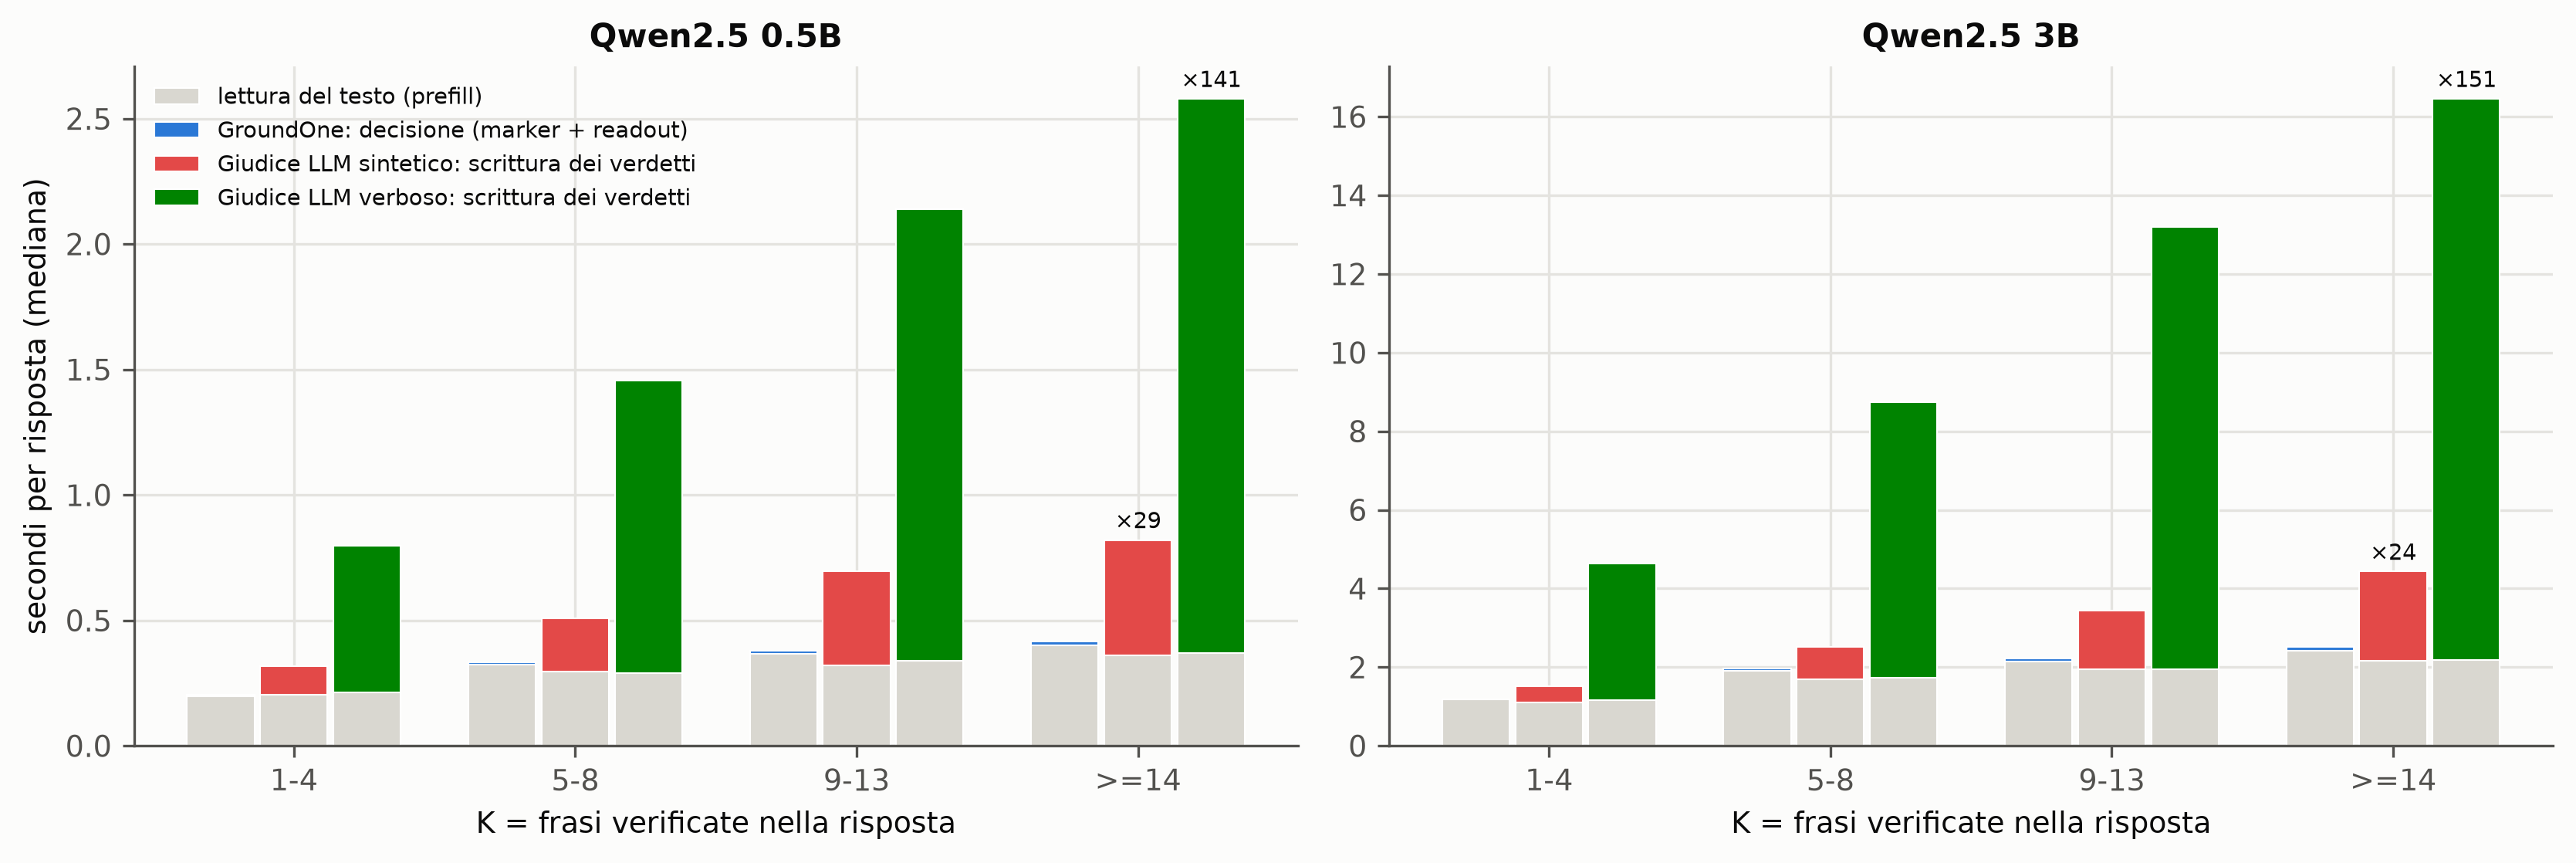
\includegraphics[width=\textwidth]{images/results/latency_split.png}
\caption{Tempo mediano per risposta scomposto in lettura del testo (prefill, in grigio, comune a ogni approccio) e
decisione (in colore), per fascia di $K$, sulle stesse 200 risposte di T1. Le etichette indicano, per $K \geq 14$,
quante volte il giudice LLM impiega più di GroundOne a decidere.}
\label{fig:results-latency-split}
\end{figure}

\paragraph{Riuso del prefisso.} La stessa misura è stata ripetuta con una parte del prompt già nella KV cache quando
parte il cronometro, la stessa per GroundOne e per i giudici LLM: le sole istruzioni, identiche per ogni richiesta
(da 63 a 81 token), oppure istruzioni e documento (circa 640 token in mediana), come accade quando una risposta
riscritta viene verificata di nuovo sulle stesse fonti (Sezione~\ref{sec:method-readout}).\footnote{Nella versione di
MLX usata per le misure (0.29.3) il kernel di attenzione fuso con maschera causale implicita restituisce risultati errati
per alcune forme quando molte query seguono chiavi già in cache, per esempio 501 token letti dopo 523 in cache. I
percorsi con prefisso in cache usano quindi una maschera causale esplicita, che coincide con un riferimento in float32;
dopo questa correzione i logit con e senza cache differiscono al più di 0.07 e le probabilità di 0.014, cioè entro
l'arrotondamento in bfloat16. Le misure senza cache, e quindi tutti gli altri risultati, non passano da questo
percorso. La versione di MLX per Swift usata dall'applicazione non presenta l'errore.} La
Tabella~\ref{tab:results-prefix-cache} riporta i tempi complessivi.

\begin{table}[htbp]
\centering
\caption{Tempo complessivo per risposta con una parte del prompt già nella KV cache, sulle stesse 200 risposte di T1:
mediane in secondi. La stessa cache vale per GroundOne e per i giudici LLM. L'ultima colonna è il rapporto fra i tempi
mediani senza cache e con il documento in cache.}
\label{tab:results-prefix-cache}
\small
\setlength{\tabcolsep}{4pt}
\begin{tabular}{llcccc}
\toprule
Modello & Sistema & \makecell{Nessun\\prefisso} & \makecell{Istruzioni\\in cache} & \makecell{Documento\\in cache} & \makecell{Risparmio con\\il documento} \\
\midrule
0.5B & GroundOne & 0.342 & 0.333 & 0.108 & 3.2$\times$ \\
 & Giudice LLM sintetico & 0.673 & 0.652 & 0.520 & 1.3$\times$ \\
 & Giudice LLM verboso & 1.826 & 1.844 & 1.683 & 1.1$\times$ \\
\midrule
3B & GroundOne & 2.002 & 1.913 & 0.583 & 3.4$\times$ \\
 & Giudice LLM sintetico & 3.102 & 3.002 & 1.795 & 1.7$\times$ \\
 & Giudice LLM verboso & 10.277 & 9.998 & 8.742 & 1.2$\times$ \\
\bottomrule
\end{tabular}
\end{table}

Tenere in cache le sole istruzioni fa risparmiare dal 3 al 5\,\% del tempo, poco più del rumore di misura: sono il 7\,\%
dei token. Il documento, invece, è circa due terzi del prompt, e la differenza è netta. Con il documento in cache
GroundOne verifica una risposta 3.2 volte più in fretta con il 0.5B (0.11 secondi in mediana) e 3.4 volte con il 3B
(0.58 secondi). I giudici LLM guadagnano molto meno, 1.3 e 1.7 volte quello sintetico e 1.1 e 1.2 quello verboso,
perché la cache elimina soltanto la lettura e lascia intatto il decoding dei verdetti, che non si può riusare. Di
conseguenza il vantaggio di GroundOne sul giudice LLM sintetico sale da circa 2 a 4.8 volte con il 0.5B (da 4.1 a 5.2)
e da 1.6 a 3.1 volte con il 3B (da 2.8 a 3.3), e quello sul giudice LLM verboso a circa 15 volte. Sulle risposte di quattordici o più frasi, la fascia in cui la Sezione~\ref{sec:results-latency} misura lo speed-up da 1.7 a 2, il vantaggio sul giudice LLM sintetico passa a 3.6 volte con il 0.5B (da 3.5 a 3.8) e a 3.4 volte con il 3B (da 3.2 a 3.4). Con il documento in cache,
il tempo di GroundOne è fatto per il 90\,\% della lettura della sola risposta e per il resto della decisione: la verifica
di una risposta riscritta costa quindi poco più della sua lunghezza.

La velocità non è l'unica differenza (Figura~\ref{fig:results-judges}). I giudici LLM non addestrati sono anche
molto meno accurati, e non sempre rispettano il formato di output. Il giudice LLM verboso 0.5B produce un verdetto
interpretabile soltanto per il 3\,\% delle frasi, perché per lo più ricopia la risposta, mentre il giudice LLM sintetico
0.5B fallisce sul 23\,\% delle frasi. I giudici LLM 3B rispettano il formato molto meglio (0.1\,\% di errori di formato per il giudice LLM sintetico e 7.6\,\% per quello verboso), ma si fermano a una balanced accuracy a tre classi di circa 0.40, contro 0.90 del GroundOne 3B sulle stesse
risposte. Il giudice LLM verboso 3B, infine, scrive in media 248 token per risposta, che vanno tutti generati prima di poter
usare il verdetto; GroundOne, invece, non ne genera nessuno.

\begin{figure}[htbp]
\centering
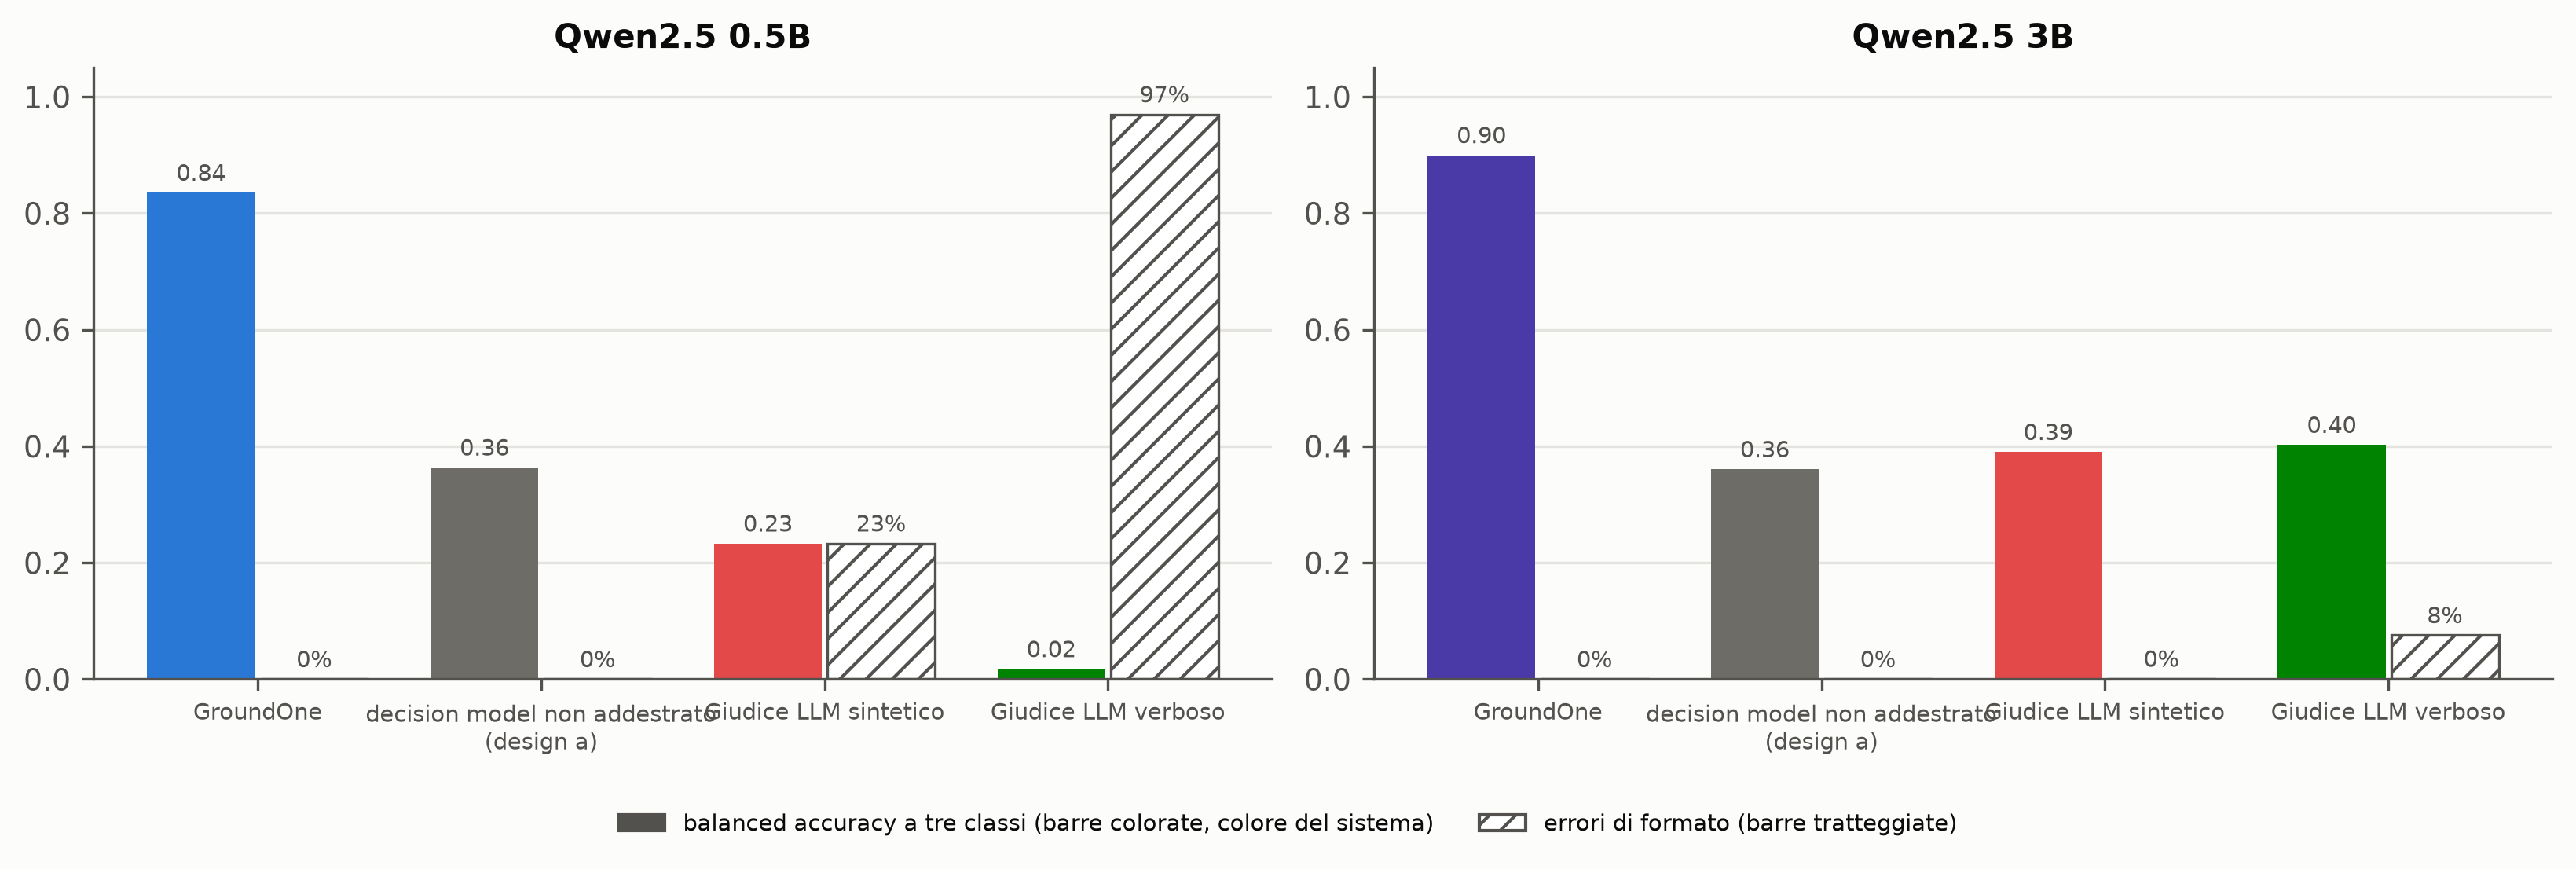
\includegraphics[width=\textwidth]{images/results/judges_quality_failures.png}
\caption{Giudici LLM sul sottoinsieme di latenza: balanced accuracy a tre classi, con gli errori di formato
contati come errori, e quota di frasi il cui verdetto non è stato possibile interpretare.}
\label{fig:results-judges}
\end{figure}

\section{Energia per verifica}
\label{sec:results-energy}

La misura dell'energia aggiunge una precisazione che la sola latenza nasconde (Figura~\ref{fig:results-energy}).
Fra i sistemi misurati, cioè GroundOne e i giudici LLM, GroundOne è quello che consuma meno energia con entrambe le dimensioni: 5.5 joule per risposta con il 0.5B e 33 con
il 3B, contro 8.9 e 43 joule del giudice LLM sintetico e 22.5 e 112 joule del giudice LLM verboso. Il suo vantaggio
sull'energia, tuttavia, è minore di quello sul tempo. Rispetto al giudice LLM sintetico, GroundOne consuma 1.6 volte meno
energia con il 0.5B e 1.3 volte meno con il 3B; rispetto al giudice LLM verboso, 4.1 e 3.4 volte meno.

Il motivo è la potenza assorbita durante il calcolo. GroundOne trascorre il suo tempo in un unico, lungo prefill, che
tiene la GPU pienamente occupata e assorbe circa 16\,W oltre la potenza a riposo. Il decoding autoregressivo dei giudici LLM,
invece, è limitato dalla banda di memoria e assorbe 11--14\,W, ma per un tempo molto più lungo. È il comportamento atteso
dalle due fasi dell'inferenza dei transformer~\cite{patel2024splitwise}, e implica che uno speed-up non vada mai letto
come un risparmio di energia equivalente~\cite{samsi2023words,luccioni2024power}.

\begin{figure}[htbp]
\centering
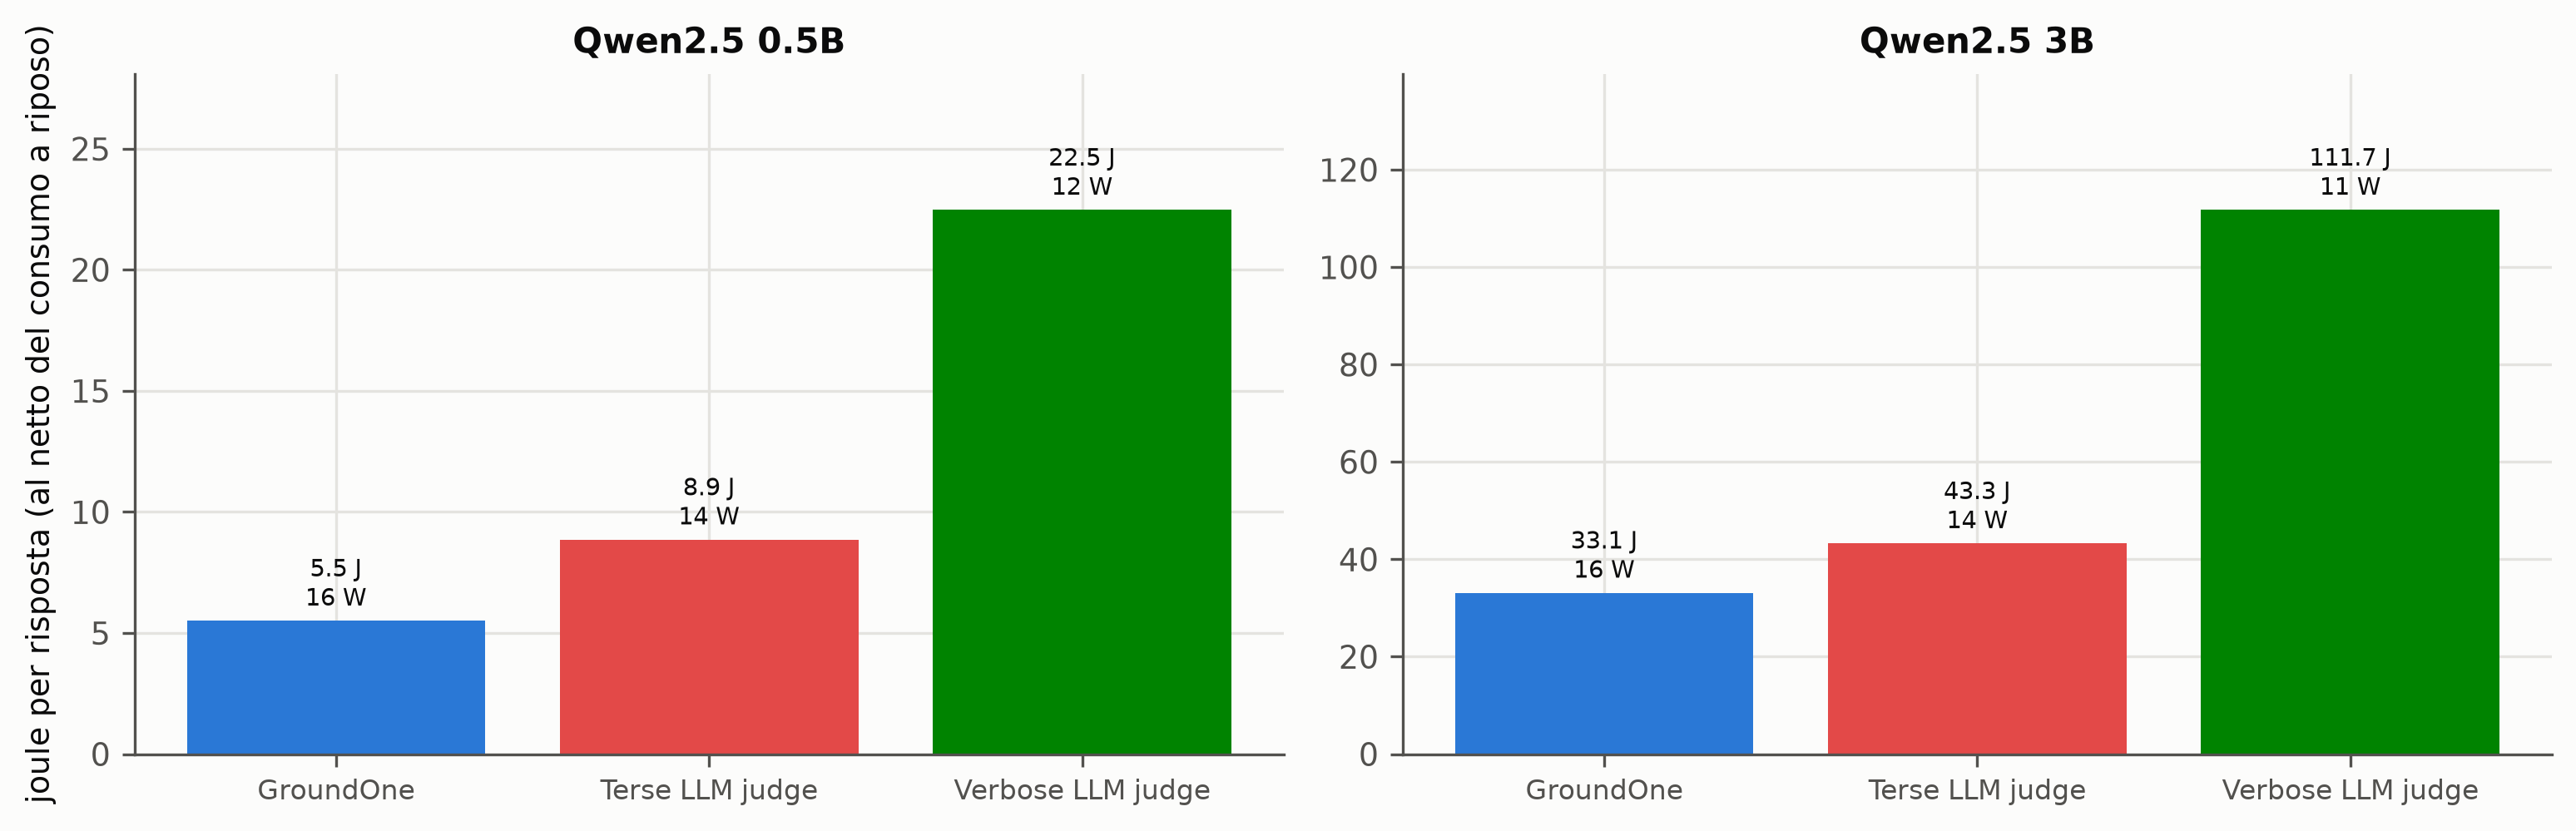
\includegraphics[width=\textwidth]{images/results/energy_per_answer.png}
\caption{Energia per risposta verificata su 100 risposte del sottoinsieme di latenza, misurata con \texttt{powermetrics} su CPU,
GPU e Neural Engine al netto della potenza a riposo, insieme alla potenza netta media durante l'esecuzione.}
\label{fig:results-energy}
\end{figure}

In termini assoluti i valori sono piccoli. Un consumo di 5.5 joule corrisponde a circa 0.0015 wattora: con l'energia di
un wattora, quindi, il GroundOne 0.5B potrebbe verificare circa seicento risposte, interamente sul portatile.

\section{Località: esecuzione offline, quantizzazione e co-residenza}
\label{sec:results-locality}

Tre misure completano il quadro del costo sul dispositivo (Sezione~\ref{sec:setup-protocol}). La prima riguarda
l'indipendenza dalla rete. La valutazione completa di T1 con il modello 0.5B, ripetuta all'interno di una sandbox che
nega al processo qualsiasi accesso alla rete, produce predizioni identiche bit per bit a quelle dell'esecuzione
originale su tutte le 17{,}284 frasi. Caricamento del modello, inferenza e valutazione non richiedono quindi alcuna
connessione. La prova è più forte di una macchina disconnessa, perché il processo non può raggiungere la rete nemmeno
quando la macchina è collegata.

La seconda riguarda la quantizzazione. Quando lo stesso adapter del 0.5B viene applicato ai pesi originali in bf16
invece che a quelli a 8 bit, le probabilità cambiano in media di 0.011 su T1 e di 0.007 su T3, e la classe predetta
coincide nel 98.3\,\% e nel 98.9\,\% delle frasi. Le metriche restano invariate: la balanced accuracy a tre classi è
0.769 con la base a 8 bit e 0.768 con quella in bf16 su T1, 0.442 in entrambi i casi su T3, e l'AUROC su T1 è 0.905
contro 0.904. La base a 8 bit, che dimezza la memoria dei pesi, non costa quindi accuratezza misurabile. La misura
riguarda però la sensibilità alla precisione della base di un adapter addestrato sulla base a 8 bit, non un modello
addestrato interamente in bf16.

La terza riguarda la co-residenza con il generatore. Nello stesso processo, il generatore Qwen2.5-3B-Instruct a 4 bit e
GroundOne verificano 30 risposte generate da documenti di T1, con una mediana di 169 token generati e di sette frasi
valutate per risposta (Tabella~\ref{tab:results-coresidence}). Con il verificatore 3B il picco di memoria allocata da MLX
è di 6.1\,GB, con il 0.5B di 3.3\,GB: entrambi ben al di sotto dei 16\,GB della macchina. La verifica occupa il
30\,\% del tempo complessivo per risposta con il 3B e il 6.7\,\% con il 0.5B. Il modello piccolo aggiunge quindi
una frazione modesta al tempo della generazione, mentre il 3B, confrontando le mediane dei due tempi, lo allunga di circa un terzo in cambio di una maggiore
accuratezza. Durante l'esecuzione con il 3B, con le normali applicazioni del desktop aperte, la memoria libera
dell'intero sistema è scesa per qualche istante a circa 1.6\,GB: la coppia sta comodamente nel processo, ma su un
portatile da 16\,GB lascia poco margine a un uso intenso del desktop. Il retriever non è incluso in questa misura; l'applicazione del Capitolo~\ref{ch:studio} lo aggiunge.

\begin{table}[htbp]
\centering
\caption{Co-residenza di generatore e verificatore in un unico processo: Qwen2.5-3B-Instruct a 4 bit come generatore,
30 documenti di T1, generazione greedy fino a 300 token. Memoria allocata da MLX; tempi mediani per risposta; la quota della verifica è la mediana delle quote per risposta.}
\label{tab:results-coresidence}
\small
\begin{tabular}{lccccc}
\toprule
Verificatore & \makecell{Memoria dopo\\il caricamento} & \makecell{Picco di\\memoria} & Generazione & Verifica & \makecell{Quota della\\verifica} \\
\midrule
GroundOne 3B & 5.0\,GB & 6.1\,GB & 4.75\,s & 1.68\,s & 30\,\% \\
GroundOne 0.5B & 2.3\,GB & 3.3\,GB & 4.65\,s & 0.28\,s & 6.7\,\% \\
\bottomrule
\end{tabular}
\end{table}

\section{Analisi degli errori}
\label{sec:results-errors}

Il risultato debole su VitaminC e le contraddizioni mancate su T1 hanno una causa comune, che la sovrapposizione
lessicale mette in evidenza. Su VitaminC, quando un'affermazione supportata condivide poche parole con la propria
evidenza (sovrapposizione inferiore a 0.4), il 0.5B la riconosce soltanto nel 2\,\% dei casi. Quando la sovrapposizione
supera 0.7, invece, la riconosce nel 64\,\% dei casi. Inoltre, il 0.5B non riconosce mai una contraddizione in
un'affermazione priva di cifre. I modelli, quindi, si appoggiano in parte alla sovrapposizione lessicale: un'affermazione
parafrasata sembra ``non menzionata'', mentre una piccola modifica a una frase copiata, spesso un numero, passa
inosservata.

La stessa debolezza si ritrova su T1, anche se con un peso minore. Quando la sovrapposizione lessicale con il documento è bassa o intermedia (fino a 0.7), la balanced accuracy a tre classi del 0.5B è 0.77. Per le frasi che riprendono dal documento più del
70\,\% delle proprie parole, invece, scende a 0.54, con una recall di 0.24 per le frasi contraddette e di 0.43 per quelle
non menzionate. Il 3B riduce questo punto cieco senza eliminarlo: sulle stesse frasi la sua recall è 0.36 e 0.56, e la
sua balanced accuracy 0.63. Le allucinazioni nascoste in frasi che per il resto ricopiano la fonte restano così il limite
principale di entrambi i modelli. VitaminC non è più difficile in assoluto: è composto in gran parte proprio da casi di
questo tipo, cioè da supporto parafrasato e da modifiche minime, che in RAGTruth sono meno numerosi.

L'Appendice~\ref{app:examples}, infine, mostra l'output di ogni sistema su una stessa risposta di esempio.
